
\documentclass[journal]{IEEEtran}

\usepackage{amsmath}
\usepackage{graphicx}
\usepackage{algorithm}
%\usepackage{algorithmic}
\usepackage{algpseudocode}
\usepackage{times} 
\usepackage{bbm}
\usepackage{amssymb}  
\usepackage{xcolor}
\usepackage{float}
\usepackage{mathtools}
\usepackage{amsthm}
\usepackage{cleveref}

\newtheorem{assumption}{Assumption}
\newtheorem{prop}{Proposition}
%\newtheorem{proof}{Proof}
%\newtheorem*{proof*}{Proof}
\newtheorem{theorem}{Theorem}
\newtheorem{lemma}{Lemma}
\newtheorem{remark}{Remarks}
\newcommand{\ttc}{\mathrm{ttc}}
\newcommand{\tts}{\mathrm{tts}}
\newcommand{\tor}{\mathrm{tor}}
\newcommand{\stp}{\mathrm{stp}}
\newcommand{\pts}{\mathrm{pts}}
\newcommand{\cta}{\mathrm{cta}}
\newcommand{\floor}[1]{\lfloor #1 \rfloor}

\newcommand{\E}{\mathrm{E}}
\newcommand{\Var}{\mathrm{Var}}
\newcommand{\argmin}{\text{argmin }}
\newcommand{\argmax}{\text{argmax }}
\newcommand\numberthis{\addtocounter{equation}{1}\tag{\theequation}}
\DeclarePairedDelimiter\ceil{\lceil}{\rceil}

% \IEEEoverridecommandlockouts

\begin{document}

\title{Urban Ridesharing with Hybrid Distributed Reinforcement Learning}

\author{Benjamin~Riviere,
        Salar~Rahili,
        and~Soon-Jo~Chung}

% make the title area
\maketitle

\begin{abstract}
Coordinating a fleet of automated taxis to optimally service urban customer requests is an anticipated challenge for Transportation Network Companies (TNC) like Uber and Lyft. In this paper, we derive a learning-based algorithm to assign taxis to customer requests to maximize long-term profit in an unknown and dynamic environment. We propose a novel, hybrid mechanism using distributed online temporal-difference (D-TD) learning with infrequent centralized Bellman updates to solve this problem in a scalable manner with regret bounds. The system is modeled as a Markov Decision Process (MDP) using customer data. The Bellman solution of the MDP is computed at a powerful central node and is passed as an initial policy to the fleet of taxis. Then, using only local information, the D-TD algorithm is computed at each taxi to capture the model errors and the environment changes, such as variations in customer demand, traffic, and fare. This solution will drift from the centralized Bellman solution, so periodically, the agents will pass their customer data to a centralized node to again exactly solve the MDP and obtain an exactly optimal centralized policy. In contrast to conventional agent-based MDP, we formulate a highly-scalable cell-based  MDP, and we exploit a game-theoretic task assignment algorithm to coordinate individual taxis, where each agent uses the optimal policy to select its customer from the set of local available requests in a distributed manner. We validate the proposed algorithm in two environments: with a simulated GridWorld and with real customer requests from the Chicago city taxi dataset. 
\end{abstract}

\begin{IEEEkeywords}
Autonomous Vehicles, Distributed Algorithms, Dynamic Programming
\end{IEEEkeywords}

\section{Introduction}
\IEEEPARstart{U}{rban} transportation plays a significant role in the development of modern cities. Almost 1.2 million deaths occur on roads each year worldwide, and reports show that $94\%$ of car accidents in the U.S. involve human errors~\cite{Google}. Autonomous cars are an emergent technology that will quickly become ubiquitous as a safer and more efficient mode of transportation. Transportation Network Companies (TNCs) are planning to deploy coordinated fleets of autonomous ground and air vehicles to improve the urban transportation capabilities~\cite{Uber}, and provide autonomous taxi services (see Fig.~\ref{overview_graphic_v2}). The deployment of a large number of agent fleets of autonomous vehicles, both ground and air, drives a coupled innovation in highly-scalable distributed algorithms. An example of an intelligent transportation network architecture is a computationally powerful central node and a large fleet of distributed taxis that operate with a small amount of processing power and communication bandwidth. In this paper, we assume this architecture and develop a framework to optimize infinite-horizon reward in a dynamic and uncertain environment.

This work develops a method to exploit the natural advantages of exact and approximate dynamic programming methods to coordinate mobile transportation agents in an urban environment. Exact methods to solve a large state-space Markov Decision Process (MDP)~\cite{bellman1957,putermanMPI} with Bellman value iteration is computationally expensive and thus cannot be computed in real-time by the individual agents. Temporal Difference Q-learning is a tractable, approximate method that bootstraps on a previous estimate and can effectively adjust to dynamic effects, such as change in customer demand or traffic. Our work develops a hybrid learning architecture that is compatible with a TNC architecture by using distributed temporal difference learning and infrequent centralized Bellman solution updates. 
\begin{figure}
\begin{center}
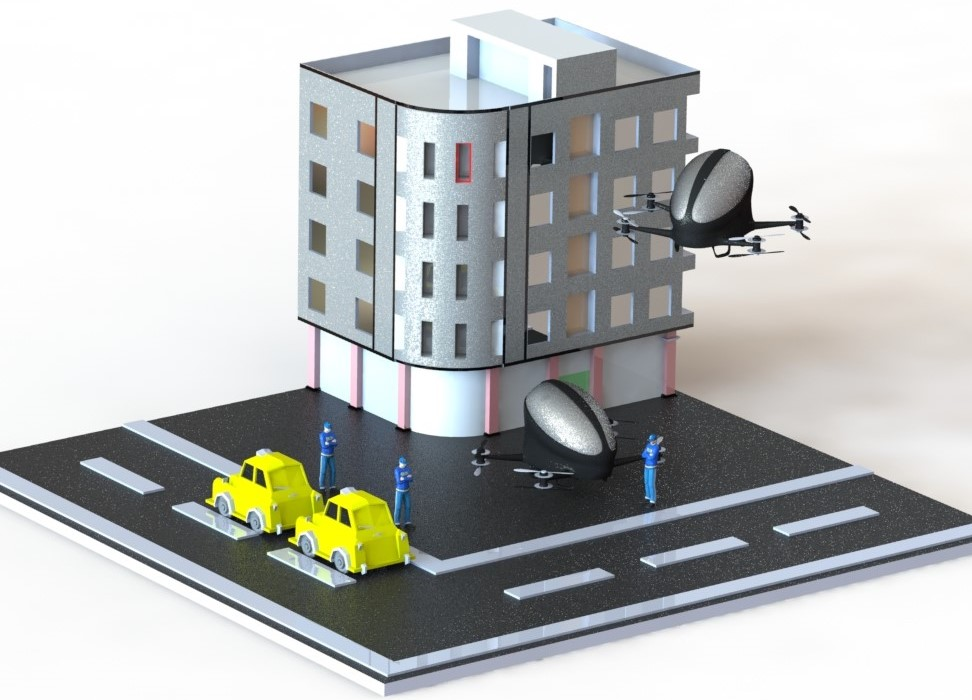
\includegraphics[width=75mm]{graphic_v3_new.jpg}
\caption{Concept graphic of an intelligent transportation network. Agents, both ground and air vehicles, estimate in real-time the state of the environment and select the customer requests to maximize the transportation company's profit.}
\label{overview_graphic_v2}
\end{center}
\end{figure}

\emph{Literature Review:} Planning such an on-demand transportation system that must adapt to customer needs in real-time has been well-studied in the literature. The problem of providing transportation services for customers can be modeled as a Pick-up and Delivery Problem~\cite{StaticSur} or its extension Dial-A-Ride Problem~\cite{DARP} in which the transportation of goods is replaced by the transportation of people. Older prior work in the literature is focused on a static routing problem, where all the customers' requests for all time are known before routes are determined. However, due to the fast dynamics of customers requests and unknown future requests, employing these methods for planning real-time transportation in urban areas is not possible. 

Recently, research has been conducted on dynamic and stochastic routing, where part or all of their input is unknown and revealed dynamically~\cite{DynHv,DynFra,DynamicSur,dynamic_congestion}. The main objective of these studies is to minimize the total distance traveled by the vehicle while servicing all customers. More sophisticated formulations~\cite{multi,Kim_2005}, are often not applicable to large-scale taxi fleets due to their centralized nature. Recent works also propose scalable solutions to dynamic routing problems. In~\cite{anticipatory_routing}, a decentralized solution is presented to minimize traffic congestion using an ant-pheromone-inspired method. In~\cite{deep_rl}, a distributed deep reinforcement-learning method is proposed to learn macro-actions in event-response. Some model-based MPC approaches include~\cite{cyber_car}, where a fleet of autonomous taxis is controlled in a scalable manner to minimize total energy cost and~\cite{schutter_2017}, where hierarchical control is used for large scale MPC. A multi-agent reinforcement learning survey paper discusses some additional methods in~\cite{schutter_2015}. All these methods used a conventional agent-based Lagrangian approach, whereas our method uses an abstracted cell-based or Eulerian method that is inherently scalable with a large number of agents, similar to the idea used in probabilistic swarm guidance~\cite{Bandyopadhyay_2017}.

Because of this abstraction, our algorithm requires an additional task assignment component to directly interface taxis with customers and to coordinate taxis. The well-known Hungarian method~\cite{kuhn, Edmonds,yu2014target}, auction-based methods~\cite{Bertsekas1988}, and parallel algorithms~\cite{Bertsekas}, and their applications in multi-robot target and task assignment~\cite{Schumacher,Jin,Bellingham} can be employed to solve our problem formulation. However, these algorithms are mainly designed to solve the assignment problem in a centralized manner. Some decentralized methods have been introduced in the literature to tackle this problem~\cite{morgan2016swarm,Dionnedec, sujitdec, How2009}. In~\cite{morgan2016swarm}, a distributed auction-based algorithm is introduced, where the task assignment problem is solved in a distributed manner. In~\cite{How2009}, the consensus algorithm is employed to find the centralized solution in a distributed manner. However, by using this approach, the size of the problem is not reduced, and only the requirement for having a central node is relaxed. As a result, the algorithm for a large number of customers and agents can become intractable. Our method employs a prescriptive game theoretic approach that is compatible with a distributed framework. Using this method, our computation time per agent does not increase with the number of agents. 

In parallel with the advances in operational routing research discussed above, the machine learning community has developed results in convergence of value iteration~\cite{littman_csaba_1998,changing,Csaba_littman_1999} useful for theoretical analysis of MDP frameworks. Applicable to our problem, there exists work characterizing the value function error due to the dynamics of a changing environment using $(\epsilon,\delta)-\mathrm{MDP}$ theory~\cite{changing}. Current advances in machine learning address the computational tractability limit associated with the curse of dimensionality for solving MDP's with a large state, control, and temporal space. This effect drives appeal for (i) function approximate methods such as deep neural networks and, in the case of multi-agent systems, (ii) distributed solutions that use only local information. Our method addresses the need for distributed learning by using distributed control theory to estimate the optimal policy. 

% Our algorithm to coordinate mobile agents in a distributed fashion to handle uncertainty in a dynamic environment is well aligned with the research directions proposed in the review study~\cite{its_review}. 

\emph{Main Contributions:} 
The overview of our algorithm is shown in Fig.~\ref{overview_algorithm}. First, we collect customer taxi data offline, and use it to formulate an MDP and solve using Modified Policy Iteration (MPI) to initialize an optimal Bellman policy. Then, we pass the optimal policy to each agent, where they each perform incremental TD online updates to capture environment dynamics and uncertainty. The agents perform distributed Q-learning using only local information and interactions to update the evolving policy. They assign customer requests cooperatively in a distributed game-theoretic task assignment, which completes the time step. If the policy update condition is met, which essentially dictates how far the agents' computed policy has drifted from the optimal policy, then the agents pass their data to the centralized node, which recomputes the MDP and corresponding MPI solution and globally re-initializes the agent's optimal policy estimates.

We borrow relevant techniques from fields of machine learning, distributed estimation, and prescriptive game theory. Our distributed reinforcement learning framework employs a one-step TD update, and allows us to derive analytical results using dynamic consensus methods developed in~\cite{DBF, saberFax2007,saber_2009}, and nonlinear stability theory using contraction~\cite{slotine_1998,slotine_contraction}. Additionally, we use results from prescriptive game theory~\cite{robust5,robust7,revisiting}, to design a potential game and iteration law to make agent action sets converge to near-optimal Nash equillibria. As compared to our preliminary work presented in the workshop article~\cite{priorWork}, this paper includes major revisions in all the sections, including a reformulation of the MDP, an update condition to iterate between exact and approximate solutions, additional mathematically-rigorous proofs of convergence, additional simulation results, and more complete proofs of the theorems. 

The main contributions of the paper are as follows: 
\begin{itemize}
    \item We present a novel agent-agnostic MDP formulation for optimal routing. In contrast with conventional agent-based methods, we decompose the program into a cell-based Markov Decision Process and we coordinate individual agents with a game theoretic task assignment. 
    \item We recast temporal difference (TD) Q-learning equations into a conventional distributed estimation theoretic framework, thereby allowing us to apply the distributed Kalman Information Filter to solve for an optimal adaptive learning rate. 
    \item We rigorously bound the error in distributed policy estimation using tracking and synchronization analysis to the TD solution. We also bound the difference between the TD solution and the Bellman solution, allowing us to derive the error of the complete Bellman solution from the distributed estimation. This regret-bound-like result permits the user of the algorithm to explicitly tune the trade-off between computational effort and performance. 
    \item We validate our results in a GridWorld simulation, and using real data from the city of Chicago taxi data set. 
\end{itemize}

The rest of this paper is organized as follows: Section~\ref{sec_math_prelim} presents notation and mathematical preliminaries. Section~\ref{sec_formulation} presents our distributed estimation formulation, convergence results, and the exact solution update condition. Section~\ref{sec_game} reviews the game theoretic formulation. Section~\ref{sec_sim_results} presents the simulation results. Concluding remarks are made in Sec.~\ref{sec_conclusion}. 
\begin{figure}
    \centering
    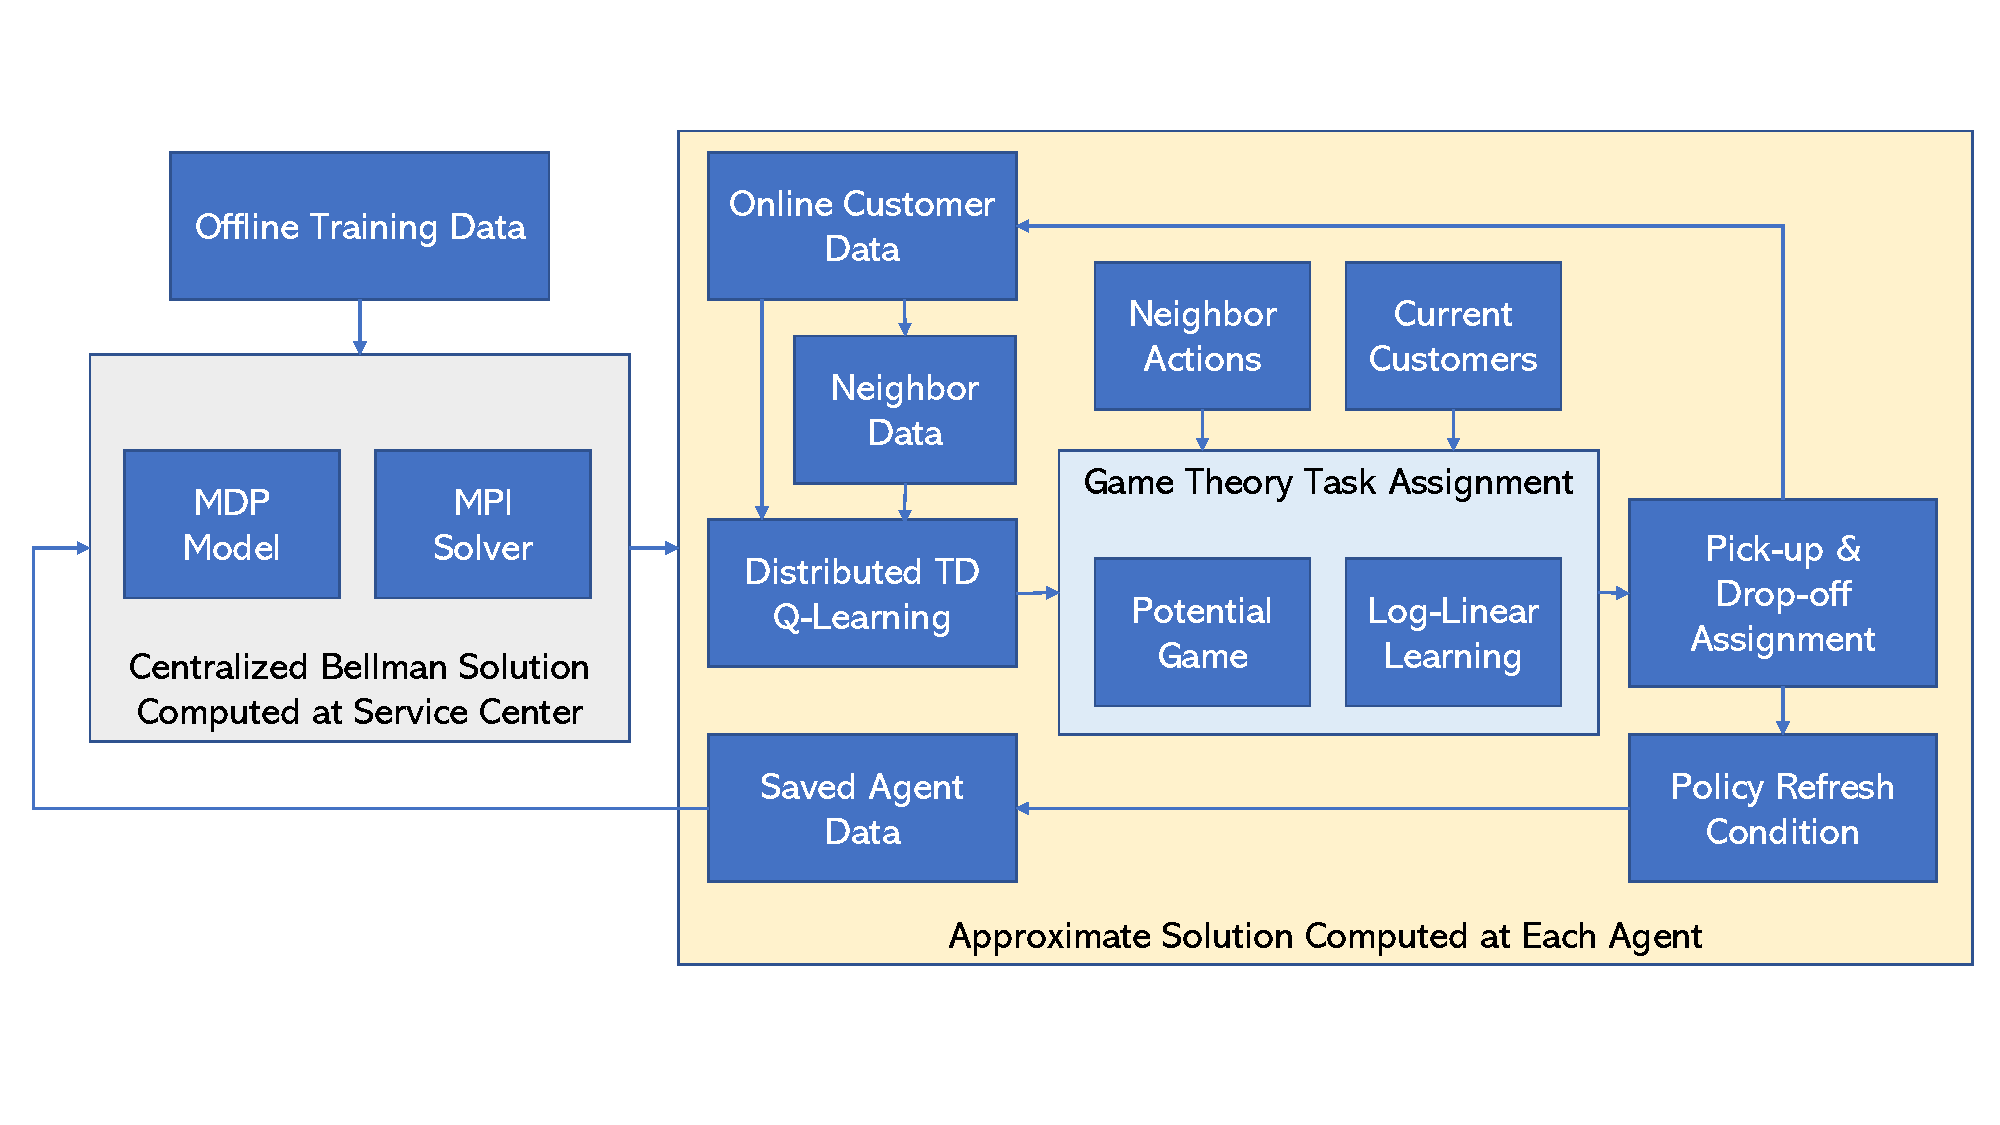
\includegraphics[width=3.5in]{overview_graphic_v3.pdf}
    \caption{Schematic of the Distributed Learning-Based Routing algorithm.}
    \label{overview_algorithm}
\end{figure}

\section{Mathematical Preliminaries} \label{sec_math_prelim}
\subsection{Notation and Definition}
Unless otherwise noted, we adopt the following conventions and notations. 
    We define objects: $\boldsymbol{1}_n = [1,...,1]^\intercal / \sqrt{n}$ and $I_n$ is the identity matrix in $\mathbb{R}^{n\times n}$ where $n$ is an arbitrary dimension.
    We define an augmented state with $[.]$. For example, $[X] = X \otimes I_{n}$, where $\otimes$ denotes the Kronecker product. 
    We denote the probability of event $s$ with $\mathbb{P}(s)$. 
    We denote the distribution of normal random variables with $\mathcal{N}(\mu, \Sigma)$, where $\mu$ is the random variable mean and $\Sigma$ is the covariance matrix. 
    Underbar denotes total infinum, $\underline{\alpha} = \inf_{t,i,(s,a)} \alpha^i_t(s,a)$ with  $0 < \underline{\alpha} \leq \alpha < 1$.
    Unless otherwise noted, $\delta$ denotes bounds and $\sigma$ denotes singular values that define contraction or convergence rates.
    We use the 2-norm.
    We denote block diagonal matrices with $\mathrm{blkdiag}(.)$. 
    The time index is denoted by $t$ subscript, the customer request index is denoted by a $k$ superscript, the superscript $i$ refers to a quantity particular to an agent.

\subsection{Markov Decision Process (MDP) Formulation}
We use a sample-based MDP formulation, where a sample is a customer request, defined as a tuple: $$c^k = \langle x^k_p, y^k_p, x^k_d, y^k_d, \mathrm{fare}^k, \ttc^k, \tor^k\rangle$$ for $k = 1,..,N_c$, where $(x^k_p,y^k_p), (x^k_d, y^k_d) \in X \subset \mathbb{R}^2$ are the pickup and dropoff coordinates of the request, $\mathrm{fare}^k \in \mathbb{R}$ is the fare of the request, $\tor^k \in \mathbb{R}$ is the time of the request, and $N_c$ is the number of customer requests. We use this tuple of data because this is the format given by the city of Chicago city data~\cite{chicagoData}. Although the position data here is in $\mathbb{R}^2$, the developed method is applicable to cells distributed in $\mathbb{R}^3$, relevant for future transportation systems including flying taxis as shown in Fig,~\ref{overview_graphic_v2}. 

In order to define the cell-based MDP tuple $\langle S,\mathcal{A},\mathcal{T},\mathcal{R},\gamma \rangle$, we need to abstract the sampled data with helper functions. We summarize descriptions for the helper functions in Table~\ref{table_helper_functions}, where the design constant $C_2$ is the average speed of taxis. We define the MDP as follows: 

\begin{table}[!t]
    \centering
    \caption{Helper Functions}
    \label{table_helper_functions}
    \begin{IEEEeqnarraybox}[\IEEEeqnarraystrutmode\IEEEeqnarraystrutsizeadd{2pt}{1pt}]{v/c/v/c/v/c/v}
        \IEEEeqnarrayrulerow\\
        &\mbox{Function}&&\mbox{Name}&&\mbox{Computation}&\\
        \IEEEeqnarraydblrulerow\\
        \IEEEeqnarrayseprow[3pt]\\
        & \cta && \text{Customer to action} &&  (\pts(x^k_p, y^k_p), \pts(x^k_d, y^k_d)) &\IEEEeqnarraystrutsize{0pt}{0pt}\\
        \IEEEeqnarrayseprow[3pt]\\
        \IEEEeqnarrayrulerow\\
        \IEEEeqnarrayseprow[3pt]\\
        & \stp && \text{State to position} && \text{Geometric centroid of map cell} &\IEEEeqnarraystrutsize{0pt}{0pt}\\
        \IEEEeqnarrayseprow[3pt]\\
        \IEEEeqnarrayrulerow\\
        \IEEEeqnarrayseprow[3pt]\\
        & \tor && \text{Time of request} && \text{Customer Data} &\IEEEeqnarraystrutsize{0pt}{0pt}\\
        \IEEEeqnarrayseprow[3pt]\\
        \IEEEeqnarrayrulerow\\
        \IEEEeqnarrayseprow[3pt]\\
        & \ttc && \text{Time to complete} && \text{Customer Data} &\IEEEeqnarraystrutsize{0pt}{0pt}\\
        \IEEEeqnarrayseprow[3pt]\\
        \IEEEeqnarrayrulerow\\
        \IEEEeqnarrayseprow[3pt]\\
        & \tts && \text{Time to start} && \tts(s, c^k) = \|\stp(s) - (x^k_p, y^k_p)\|/C_2 &\IEEEeqnarraystrutsize{0pt}{0pt}\\
        \IEEEeqnarrayseprow[3pt]\\
        \IEEEeqnarrayrulerow\\
        \IEEEeqnarrayseprow[3pt]\\
        & \pts && \text{Position to state} && \text{Cell satisfying point-in-polygon condition} &\IEEEeqnarraystrutsize{0pt}{0pt}\\
        \IEEEeqnarrayseprow[3pt]\\
        \IEEEeqnarrayrulerow
    \end{IEEEeqnarraybox}
\end{table}

\begin{itemize}
    \item $S$ is the set of states, where a state is defined as a cell index of a discretized map. The states are discretized according to their spatial coordinates, $(x,y) \in X \subset \mathbb{R}^2$. 
    \item $\mathcal{A}$ is the set of actions, $a\in\mathcal{A}$, where an action defined as moving to a pick-up state, then moving to drop-off state. We can parameterize the action as $a = (s_p, s_d)$
    \item $\mathcal{T}$ is the transition probability function. $\mathcal{T}:S \times \mathcal{A} \times S \rightarrow \mathbb{P}$, $\mathcal{T}(s,a,s') = \mathbb{P}(s' | s,a)$. For our application, we have a deterministic transition, $\mathcal{T}(s,a,s') \in \{0,1\}$. Multiplication by the transition probability function extracts the quantity at the next state following the given action. 
    \item $f(s,a)$ is the transition function that maps a state-action pair to the next state $s'=f(s,a)$ so that $f: S \times \mathcal{A} \rightarrow S$, where $s'$ corresponds to the drop-off state of a customer request, which can be any state in $S$. We use this function for the definition of $\mathcal{T}$:
    \begin{align*}
        \mathcal{T}(s,a,s') =
        \begin{cases}
        1 & f(s,a) = s' \\ 
        0 & \mathrm{else}
        \end{cases}
    \end{align*}
    \item $\mathcal{R}(s,a)$ is the reward function returning the profit of a state-action pair: $\mathcal{R}:S \times \mathcal{A} \rightarrow \mathbb{R}$. For a single customer request, we can calculate a sample reward instance: 
    \begin{align}
        \label{eq:mdp_instant_reward}
        r^k(s,c^k) = \mathrm{fare}^k - C_1 \tts(s,c^k) - C_1 \ttc^k
    \end{align}
    where the constant design parameter $C_1$ is the cost per time. For example, in the Chicago city taxi simulation, we set $C_1$ to be 1 cent per second. 
    We derive the MDP reward, $\mathcal{R}_t$ at time $t$ by batch averaging the data set of previous customer requests reward information, with a geometric penalty to discount outdated information:
    \begin{align*}
        \mathcal{R}_t(s,a) &= \frac{ \sum_{k = 1}^{ N_c} \lambda^{\tor^k - t} \mathcal{I}(\cta( c^k) = a) r^k(s,c^k) }{ \sum_{k = 1}^{ N_c} \lambda^{\tor^k - t} \mathcal{I}(\cta( c^k) = a)}
    \end{align*}
    where $\mathcal{I}$ is the indicator function, $\lambda$ is a design parameter, and we only consider samples taken before time $t$.
    We chose the reward to be the TNC's company profit, but this choice is arbitrary and we could use the conventional reward function that minimizes customer waiting time. % : $\mathcal{R}(s,a) = -(\tor - \tts(s,a))$. 
    \item $\gamma$ is the discount factor and $0 < \gamma < 1$.
\end{itemize}

 Inherently, the sample-based MDP will become the true optimal policy as the number of samples goes to infinity. At a given time, $t$, we can calculate the exact solution of the MDP as a set of optimal policies, $\pi_t^*$ that maps from state to the optimal action using a modified policy iteration (MPI). In this paper, we consider the solution of the sampled-MDP as our optimal baseline that we attempt to estimate, because we define our base MDP with sampled information. 

Note that we do not adopt a conventional multi-agent MDP framework for a vehicle routing problem with stochastic service requests, as suggested in~\cite{ulmer_2018}. Instead, our MDP is a framework is agnostic to the number of agents, and the value function it provides simply captures the value of a cell in the map for a given customer dataset. In effect, the computational complexity scales with the number of cells in the environment, not the number of agents. Our MDP formulation is inspired from an fluid mechanics `Eulerian' perspective,~\cite{Bandyopadhyay_2017}, compared with the conventional agent-based 'Lagrangian' MDP formulation. The action space of the MDP, $\mathcal{A}$, is an abstraction of the taxi's real behavior to pickup and dropoff customers. In Sec.~\ref{sec_game}, we complement this approach by hierarchically constructing an agent-based game that directly interfaces customers with taxis. 

\subsection{Q-learning Formulation}
Reinforcement learning describes a set of methods that can be used to solve a general problem of simultaneously finding near-optimal solutions while exploring an unknown environment. In the urban taxi dynamic assignment problem, the reward model, $\mathcal{R}(s,a)$ is unknown and dynamically affected by the revenue, $\mathrm{fare}^k$, which is driven by customer demand, and by the time to complete task, $\ttc$, which is driven by traffic hours. Both of these values are unknown and time-varying, and we estimate this information by sampling actions and making measurements in the environment. In this paper, we alternate between two Q-learning methods: Bellman iteration and temporal difference (TD). In both cases, the reinforcement learning algorithms are attempting to estimate and maximize the value function: 
\begin{align*}
    V(s) &= \max_a (\mathcal{R}(s,a) + \gamma \sum_{s'} \mathcal{T}(s,a,s') V(s'))
\end{align*}

First, we present the standard Bellman Q-iteration~\cite{SuttonB98}, denoted by $Q^*$. We capture the net effect of customer demand and traffic through a time-varying optimal $Q$ value, defined by the Bellman optimality equation, and we simplify using the deterministic transition function: 
\begin{align*}
    Q^{*}_t(s,a) &= \mathcal{R}_t(s,a) + \gamma \max_{a' \in \mathcal{A}} Q^{*}_t(f(s,a),a')
\end{align*}
where $Q_t^*: S \times \mathcal{A} \rightarrow \mathbb{R}$ and we take the maximum over actions $a'$. We apply a tabular Q value setting, where elements correspond to state action pairs, and we flatten the matrix into a vector such that $Q^{*}_t \in \mathbb{R}^{n_q}$ where $n_q = |S| |\mathcal{A}| = |S|^3$ and $|S|$ is the number of cells. Additionally, we take the environment to be dynamic, so we add a subscript $t$ to the $Q^*_t$ and $\mathcal{R}_t$ vector. We denote the $Q^*_t$ vector with no argument, and an element of $Q^*_t$ vector with a state-action argument. In vector form, we can write the Bellman Q-iteration as:
\begin{align}
    \label{eq:bellman_q}
    Q^{*}_t &= \mathcal{R}_t + \gamma \mathcal{T} Q^*_t
\end{align}
where $\mathcal{T}$ is the MDP transition function. 

Next, we discuss the model-free, temporal difference (TD), one-step Q-learning~\cite{SuttonB98}, denoted here $Q^{**}_t$. We receive information via sampled actions from taking customer requests. Then we can calculate an instance of the reward function, $r^k_t = \mathcal{R}_t + v_t$ where $v_t \sim \mathcal{N}(0, \Sigma_t)$ is the measurement noise, and estimate $Q^{**}_t$ with the following conventional TD method: 
\begin{align}
    Q^{**}_{t+1} &= (I-\alpha^{**}_t H^{**}_t) Q^{**}_{t} + \alpha^{**}_t H^{**}_t (\mathcal{R}_t + v_t + \gamma \mathcal{T} Q^{**}_t)
    \label{eq:td_q}
\end{align}
where $\alpha^{**}_t \in \mathbb{R}^{n_q \times n_q}$ is the learning rate and $H^{**}_t$ is the measurement model for the available measurements. We define diagonal matrix $H^{**}_t \in \mathbb{R}^{n_q \times n_q}$ to be the average measurement model of all agents, if the information was perfectly centralized:
\begin{alignat}{2}
    \label{eq:td_measurement}
    H^{**}_t &= [\boldsymbol{1}]^\intercal [H]_t [\boldsymbol{1}] \\ 
    [H]_t &= \mathrm{blkdiag}( H^1_t, ..., H^{n_i}_t) \nonumber \\ 
    H^i_t(j,j) &= \begin{cases}
        1 & \mathrm{if} \ \ M_t(i,j) = 1 \\
        0 & \mathrm{else}
    \end{cases} \nonumber 
\end{alignat}
where $n_i$ is the number of agents, $M_t \in \mathbb{R}^{n_i \times n_q}$ is an activation function obeying $M_t(i,j) = 1$ if and only if agent $i$ has a measurement at state-action index $j$ at time step $t$. Similarly, we define the TD-learning  rate as: 
\begin{align}
    \label{eq:td_learning_rate}
    \alpha^{**}_t &= [\boldsymbol{1}]^\intercal [\alpha]_t [\boldsymbol{1}] \\ 
    [\alpha]_t &= \mathrm{blkdiag}( \alpha^1_t, ..., \alpha^{n_i}_t) \nonumber
\end{align}
where $[\boldsymbol{1}] \in \mathbb{R}^{n_i n_q \times n_q}$, $\alpha_t^i \in \mathbb{R}^{n_q \times n_q}$ and $[\alpha]_t \in \mathbb{R}^{n_i n_q \times n_i n_q}$, and we define the individual agent learning rates, $\alpha^i_t$ in Section~\ref{subsec:distributed online learning}. 

We have added the measurement model to the conventional Bellman and TD equations and written in vector form. In our framework, each agent estimates the optimal policy, $\hat{Q}^i_t$ by solving~\eqref{eq:bellman_q} with a Modified Policy Iteration (MPI) and initializing to the Bellman value, $\hat{Q}^i_0 = Q^*_0$. Then, we account for the changing environment by updating the $\hat{Q}^i_t$ value online with a low-computational cost, incremental temporal difference~\eqref{eq:td_q} at each timestep at each agent. The Bellman method computes with a batch process, and it is computationally expensive thus cannot be evaluated at each timestep by each agent. The TD learning technique works naturally with incremental data and is especially effective because we start from an optimal policy, so we are 'bootstrapping' onto an already close-to-optimal policy. In our formulation, we decentralize the TD learning and compute a distributed estimation at each agent. 

\subsection{Assumptions}
We make the following assumptions about our system: 
\begin{assumption}
    \label{assumption: connected}
    The communication graph of taxis is connected at all times, i.e., $\lambda_2(L) > 0$, where $\lambda_2$ denotes the second eigenvalue and $L$ is the communication graph Laplacian matrix (mathematically defined in Sec.~\ref{sec_formulation}). 
\end{assumption}
\begin{assumption}
    \label{assumption: balanced}
    The communication graph of taxis is balanced, i.e., $\boldsymbol{1}^\intercal L = \boldsymbol{0}$
\end{assumption}
\begin{assumption}
    \label{assumption: bounded_changing_environment}
    The dynamics of the environment is bounded such that there exists a constant that bounds the rate of change of the policy: $$\exists \delta_\mathrm{e} \ \ \mathrm{s.t.} \ \ \delta_\mathrm{e} = \sup_{t} \| \mathcal{R}_t + \gamma \mathcal{T} \hat{Q}^i_t - \hat{Q}^i_{t} \|$$ 
\end{assumption}
\begin{assumption}
    \label{assumption: periodic_full_measurement}
    Every state action pair, $(s,a)$ is sampled by at least one agent every $\boldsymbol{T}$ timesteps. 
\end{assumption}
Assumption~\ref{assumption: connected} is appropriate for an urban environment because, with a large spatial density of taxis, the communication graph is guaranteed to stay connected. Assumption~\ref{assumption: balanced} is trivially satisfied by our use of an undirected communication graph. Assumption~\ref{assumption: bounded_changing_environment} is the difference between the measurement and current state, and this assumption is bounding the change in the environment in time, which implies there are no shocks in the reward and transition model, which is a proper assumption as no terms in the reward model can go unbounded. Assumption~\ref{assumption: periodic_full_measurement} is reminiscent of an adaptive control Collective Sufficient Richness requirement~\cite{slotine_cloud}, where the reference signal needs to have enough information to converge on a parameter estimation. This assumption is appropriate for system with a large ratio of the number of agents (and samples) to number of states, and with a large exploration/exploitation trade-off value.

\section{Main Results Hybrid Distributed Learning} \label{sec_formulation}
In the first subsection, we present a solution to this problem where the control/estimation is all processed through a central node, corresponding to the conventional TD result. Then, we present a distributed formulation extension and the distributed performance bounds, with respect to TD and Bellman optimal policy. 
\subsection{Centralized TD-Learning}
We consider the state of the system as augmented position and Q-values, and perform online estimation techniques on the Q-values, while assuming full knowledge of self state, $s$. By formulating the Q-learning iteration as a linear dynamical system, we apply the Kalman Information Filter (KIF) or its multi-agent form~\cite{DBF} to optimally estimate within one-step TD iteration. Formulating the Q-learning iterations~\eqref{eq:bellman_q}~\eqref{eq:td_q} with conventional control theory, and assuming zero-mean Gaussian noise, we arrive at the following canonical equations for the estimator and measurement:
% DISCRETE TIME
\begin{align}
    Q^{**}_{t+1} &= Q^{**}_t + \alpha^{**}_t ( z^{**}_t - H_t^{**} Q^{**}_t) \label{eq:td_dynamics} \\
    z^{**}_t &= H^{**}_t (\mathcal{R}_t + \gamma \mathcal{T} Q^{**}_t + v_t) \label{eq:td_update}
\end{align}
where $\alpha^{**}_t$ is the learning rate for each state-action pair, $\alpha^{**}_t \in \mathbb{R}^{n_q \times n_q}$, $z^{**}_t$ is the pseudo-measurement update vector, as the direct measurements are the set of $\mathcal{R}_t + v_t$ that we augment with the previous estimation. The measurement noise is denoted by $v_t \sim \mathcal{N}(0,\Sigma_t) \in \mathbb{R}^{n_q}$, $H^{**}_t$ is the measurement model, and $\Sigma_t$ is the measurement noise covariance matrix, upper bounded by $\varsigma I$. We model the TD equations~\eqref{eq:td_dynamics} and~\eqref{eq:td_update} directly from~\eqref{eq:td_q}. 

\subsection{Distributed Online Learning: State Sharing}
\label{subsec:distributed online learning}
The centralized formulation in the previous section guarantees optimal estimation of $Q$ values for a single TD step. However, in considering computational and hardware limitations of the autonomous fleet, it is important to develop distributed algorithms that only use local information. The governing equations for the distributed system are similar, except we add a superscript $i$ that denotes the equations are solved in a distributed fashion at each agent, $i = 1,...,n_i$. 

The conventional Distributed KIF~\cite{DBF} uses a measurement-sharing scheme where a dynamic consensus algorithm is used to average measurements and covariance matrices after being transformed by the information filter change of basis. We consider another form of the distributed Kalman filter with a state-sharing scheme (i.e., agent $i$ shares $\hat{Q}^i_t$) with the dynamic consensus outside of the innovation step of the Kalman filter.
% Discrete time
\begin{align}
    \hat{Q}_t^i &= \hat{Q}_{t-1}^i + \alpha_t^i ( z_t^i - H_t^i \hat{Q}_{t-1}^i) \label{eq:agent_dist_dynamics} \nonumber \\
    & \ \ \ \ \  + \sum_j A_t(i,j) (\hat{Q}_{t-1}^j - \hat{Q}_{t-1}^i) \\
    z_t^i &= H^i_t (\mathcal{R}_t + \gamma \mathcal{T} \hat{Q}^{i}_t + v_t) 
    \label{eq:z_dist}
\end{align}
where $H^i_t$ is defined as in the centralized case, except activation function $M_t(i,j)$ is evaluated only at the index of the agent performing the update and $A_t$ is the time-varying, doubly stochastic adjacency matrix, defined in~\cite{DBF}. We stack the dynamics as follows for our analysis: 
\begin{align}
    [\hat{Q}]_t &= (I - [\alpha]_t [H]_t - [L]_t) [\hat{Q}]_{t-1} + [\alpha]_t [z]_t \label{eq:stacked_dist_ss}
\end{align}
where the dimension of the equation is $\in \mathbb{R}^{n_i n_q \times 1}$ and $[\hat{Q}]_t = [\hat{Q}_t^1; ...; \hat{Q}_t^{n_i}]^\intercal$, $[\alpha]_t = \mathrm{diag}[\alpha_t^1, ..., \alpha_t^{n_i}] \in \mathbb{R}^{n_i n_q \times n_i n_q}$, $[L]_t \in \mathbb{R}^{n_i n_q \times n_i n_q}$. Here, $L_t \in \mathbb{R}^{n_i \times n_i}$ is the time-varying Laplacian matrix of the graph, defined as $L_t = I-A_t$. Additionally we augment this matrix using the kronecker product: $[L]_t = L_t \otimes I_{n_q}$. For the measurement model, $[H]_t$, the stacked model is a diagonal matrix of each of the agents measurements models, i.e., $[H]_t = \mathrm{blkdiag}[H_t^1, ..., H_t^{n_i}]$. Note that these measurement models are switching, heterogeneous, and time-varying, and the flexible nature of contraction analysis allows us to deal with it naturally. Finally, the measurement is stacked as $[z]_t = [z_t^1; ...; z_t^{n_i}]^\intercal$, and note that:
\begin{align}
    \label{eq:z_stacked_update}
    [z]_t &= [H]_t ([\boldsymbol{1}]\mathcal{R}_t + [\boldsymbol{1}] v_t + \gamma [\boldsymbol{1}] \mathcal{T} [\boldsymbol{1}]^\intercal [\hat{Q}_{t-1}])
\end{align}

Additionally, we can model the effect of the changing environment on the Bellman optimal solution as process noise. 
\begin{align}
    Q^{*}_{t+1} &= Q^{*}_{t} + w_t \nonumber 
\end{align} 
where $w$ is a normal random variable representing the process noise that corresponds to the changing environment, $w_t \sim \mathcal{N}(0,\mathcal{W}_t) \in \mathbb{R}^{n_q}$. With knowledge of the changing MDP model, we can tune the process noise covariance, $\mathcal{W}_t$, to match the dynamics of the MDP. For example, in the transition to rush hour times, the MDP-dynamics are fast, and we can increase the process noise such that the agents have a more aggressive learning rate and weigh their measurements more. 

In this form, we can employ the Kalman filter or KIF~\cite{DBF} to optimally choose the learning rate, $\alpha^i_t$ to estimate $Q_t^{*}$. 
\begin{align}
    \label{eq:optimal_alpha}
    \alpha^i_t &= P^i_{t|t-1} (H^i_t)^\intercal (S^i_t)^{-1}
\end{align}
where $P^i_{t|t-1}$ and $S^i_t$ are defined in the Appendix, Sec.~\ref{sec: KIF}. At each time step, each agent, $i$, receives a measurement for their customer service, i.e., $\mathrm{fare}, \ttc$, which we then transform into a pseudo-measurement update vector for each agent, $z^i_t$, using \eqref{eq:z_dist} to evaluate the KIF. We fuse the local agents state outside the measurement update. It is a known result from control theory that the optimal learning rate for this system is the Kalman gain (see the definition of KIF in Appendix, Sec.~\ref{sec: KIF})~\cite{saberFax2007,saber_2009}. The Kalman gain depends on the measurement covariance, $\Sigma_t$, process covariance, $\mathcal{W}_t$, and each agent's propagated error covariance. By re-casting Q-learning iteration equations into a conventional distributed estimation theoretic framework, we can apply the Kalman Information Filter and solve the Kalman Gain as an optimal adaptive learning rate. In the machine learning community, developing an optimal adaptive learning rate is an active area of research. To summarize the different policy evolutions, we refer to Fig.~\ref{fig:diff_q}.
\begin{figure}
    \centering
    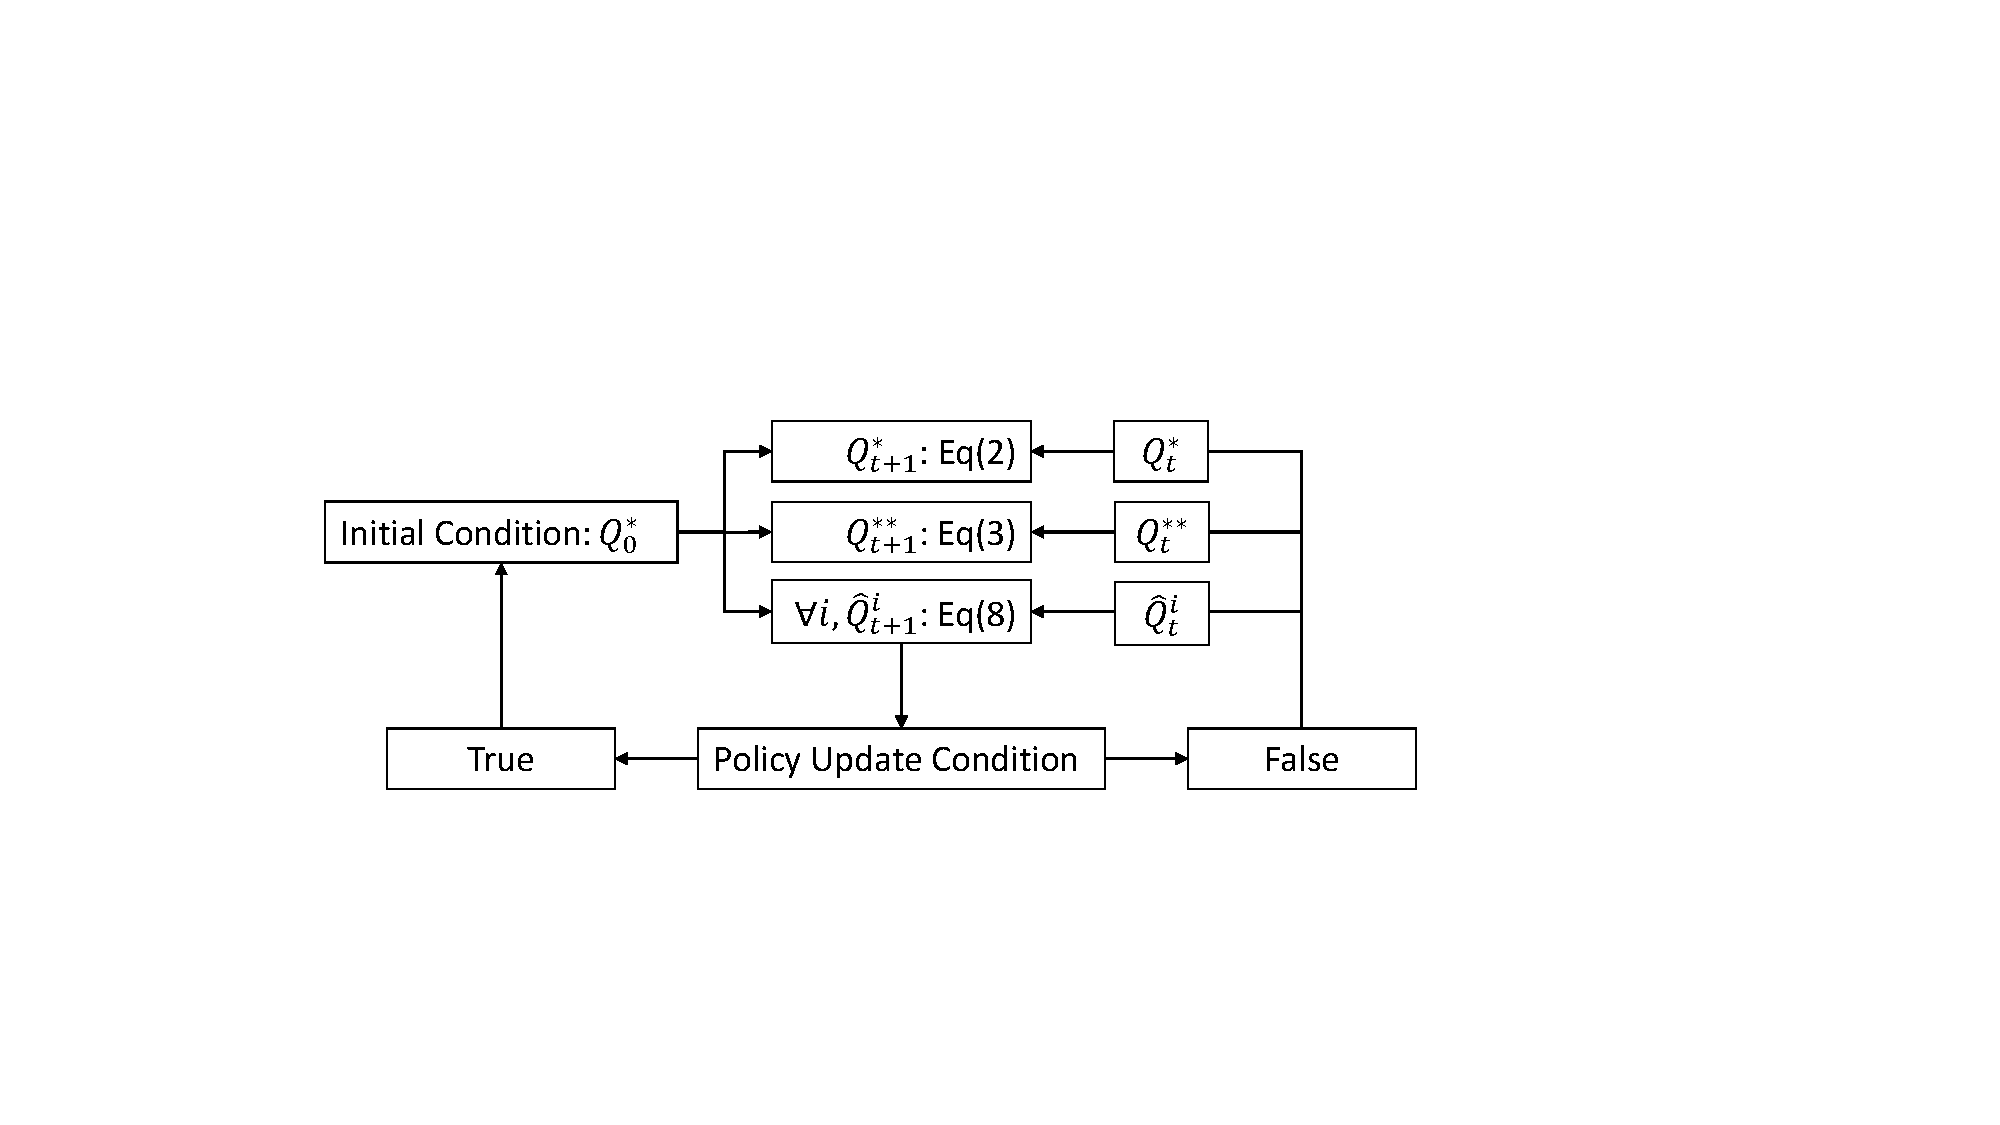
\includegraphics[scale = 0.4, trim={4cm 5cm 5cm 4cm}, clip]{different_q_block_diagram.pdf}
    \caption{Summary Block Diagram for different $Q$ policy dynamics}
    \label{fig:diff_q}
\end{figure}

The performance bounds are presented here: in Theorems~\ref{result:synch},~\ref{result:tracking}, and~\ref{result:t+s}, we compare agent's distributed policy estimation against the TD-optimal policy, $Q_t^{**}$. In Theorem~\ref{thm:hybrid_rl}, we compare the two learning methods: TD and Bellman, which lets us present the main result, Theorem~\ref{result:policy_update}, comparing the agent's distributed policy estimation to the Bellman solution, $Q_t^*$. Our analysis builds on the Discrete Gronwall Lemma, Theorem~\ref{thm:discrete_gronwall}, included in Appendix for completeness, and Theorem 1 of~\cite{Pham08} for discrete stochastic contraction. We use this result for a robust discrete contraction result, where  discrete contraction defines the largest singular value of the Jacobian as the rate of contraction of the system (`$C$' in the Gronwall lemma) and the Gronwall lemma defines the bound of the sequence. 

\begin{theorem}
    \label{result:synch}
    The state $[\hat{Q}]_t$ exponentially converges to the synchronization manifold, $[V_s]^\intercal [\hat{Q}]_t = 0$, at contraction rate $\sigma_\mathrm{s}$, within a bound, $\delta_\mathrm{s}$, implying each agent's estimate converges to the synchronized value within the same error bound. 
    \begin{align*}
        \sigma_\mathrm{s} &\triangleq 1 - \inf_{t'} \lambda_2(L_{t'})  \\
        \delta_\mathrm{s} & \triangleq \frac{ n_i \delta_\mathrm{e}}{ \inf_{t'} \lambda_2(L_{t'})} \\ 
        \| \hat{Q}_t^i - [\boldsymbol{1}]^\intercal \hat{Q}_t\| &\leq \delta_\mathrm{s}( 1 - \sigma_\mathrm{s}^t) 
    \end{align*}
    where the synchronization manifold, $[V_s]^\intercal [\hat{Q}]_t = 0$, is defined by augmenting the eigenbasis of the Laplacian matrix, $L_t$, where $L_t V_t = D_t V_t$, $V = [ \boldsymbol{1}, V_s]$ and $D_t$ is a diagonal matrix of eigenvalues. 
\end{theorem}

\begin{IEEEproof}
    We transform \eqref{eq:stacked_dist_ss} by the eigenbasis of the augmented Laplacian: $[V]: [L][V] = [\Lambda] [V]$, $[V] = [ [\boldsymbol{1}], [V_s]]$:
    \begin{align*}
        &    
        \begin{bmatrix} 
            I - [\boldsymbol{1}]^\intercal [\alpha]_t [H]_t [\boldsymbol{1}] & -[\boldsymbol{1}]^\intercal [\alpha]_t [H]_t [V_s] \\
            - [V_s]^\intercal [\alpha]_t [H]_t [\boldsymbol{1}] & [V_s]^\intercal ( I - [\alpha]_t [H]_t - [L]_t) [V_s] 
        \end{bmatrix} \cdot \\ 
        & \ \ \ \ \begin{bmatrix}
            [\boldsymbol{1}]^\intercal [\hat{Q}]_{t-1} \\ [V_s]^\intercal [\hat{Q}]_{t-1}
        \end{bmatrix} 
        + \begin{bmatrix}
            [\boldsymbol{1}]^\intercal [\alpha]_t [z]_t \\ [V_s]^\intercal [\alpha]_t [z]_t
        \end{bmatrix}= \begin{bmatrix}
            [\boldsymbol{1}]^\intercal [\hat{Q}]_{t} \\ [V_s]^\intercal [\hat{Q}]_{t}
        \end{bmatrix}
    \end{align*}
    where $[\boldsymbol{1}]^\intercal [L]_t = 0$ by the balanced graph assumption (Assumption~\ref{assumption: balanced}), $[L]_t [\boldsymbol{1}] = 0$ by definition, and $[\boldsymbol{1}]^\intercal [V_s] = [V_s]^\intercal [\boldsymbol{1}] = 0$ by orthogonality of the Laplacian eigenbasis. \newline
    Consider the state projected in the $[V_s]$ directions:
    \begin{align*}
        [V_s]^\intercal [\hat{Q}]_t &= [V_s]^\intercal ( I - [\alpha]_t [H]_t - [L]_t)[V_s][V_s]^\intercal [\hat{Q}]_{t-1} \\  
        & -[V_s]^\intercal [\alpha]_t [H]_t [\boldsymbol{1}] [\boldsymbol{1}]^\intercal [\hat{Q}]_t + [V_s]^\intercal [\alpha]_t [z]_t
    \end{align*}
    We apply the orthogonality identity, $ [\boldsymbol{1}] [\boldsymbol{1}]^\intercal + [V_s] [V_s]^\intercal = I$, to reduce to:
    \begin{align*}
        [V_s]^\intercal [\hat{Q}]_{t} &= [V_s]^\intercal ( I - [L]_t) [V_s] [V_s]^\intercal [\hat{Q}]_{t-1} + \\
            & [V_s]^\intercal [\alpha]_t ( [z]_t - [H]_t [\hat{Q}]_{t-1})
    \end{align*}
    We apply partial contraction results and consider virtual system for $y$:
    \begin{align*}
        y_t &= [V_s]^\intercal ( I - [L]_t)[V_s] y_{t-1} + d_t \\ 
        d_t &= [V_s]^\intercal [\alpha]_t ( [z]_t - [H]_t [\hat{Q}]_{t-1})
    \end{align*}
    The unperturbed system, $d_t = 0$, admits solutions $y_t = [V_s]^\intercal \hat{Q}_{t}$ and $y = 0$, so a contracting system will imply exact, global exponential convergence to the synchronization manifold, within a bound determined by the disturbance $d$. The Jacobian is given as: $ [V_s]^\intercal ( I - [L]_t) [V_s]$. Note that $[V_s]^\intercal [L][V_s] = [D_s]$, where $D_s$ is a positive definite matrix of eigenvalues of $L$, where the smallest eigenvalue of $L$ is nonzero by Assumption~\ref{assumption: connected}.
    \begin{align*}
        \sigma_1 &\leq 1 - \inf_{t'} \lambda_2(L_{t'}) \triangleq \sigma_s
    \end{align*}
    where $\lambda_2(L)$ is the Fiedler value of the communication graph. We reduce the disturbance by Assumption~\ref{assumption: bounded_changing_environment}, apply Discrete Gronwall, Theorem~\ref{thm:discrete_gronwall}, and remove the decaying initial condition as the agents are initialized with the same policy:
    \begin{align*}
        \| [V_s]^\intercal \hat{Q}_{t} \| &\leq \frac{ n_i \delta_\mathrm{e}}{ \inf_{t'} \lambda_2(L_{t'})}( 1 - \sigma_s^t)
    \end{align*}
    Additionally, note that the bound trivially holds for a single agent, and is less tight:
    \begin{align*}
        \| \hat{Q}_t^i - [\boldsymbol{1}]^\intercal \hat{Q}_t\| & \leq \| \hat{Q}_t - [\boldsymbol{1}] [\boldsymbol{1}]^\intercal \hat{Q}_t\| = \|[V_s] [V_s]^\intercal \hat{Q}_t\| \\
        &\leq \|[V_s]^\intercal \hat{Q}_t\| 
    \end{align*}
\end{IEEEproof}

\begin{theorem}
    \label{result:tracking}
    The agent's synchronized value, $[\boldsymbol{1}]^\intercal \hat{Q}_t$ corresponds exactly to the TD-optimal policy, $Q^{**}_t$ for all time $t$. 
\end{theorem}

\begin{IEEEproof}
    \label{proof:tracking}
    Projecting the stacked dynamics~\eqref{eq:stacked_dist_ss} into the centroid directions:
    \begin{align*}
        [\boldsymbol{1}]^\intercal [\hat{Q}]_t &= [\boldsymbol{1}]^\intercal(I - [\alpha]_t [H]_t) [\boldsymbol{1}] [\boldsymbol{1}]^\intercal [\hat{Q}]_{t-1} + [\boldsymbol{1}]^\intercal [\alpha]_t [z]_t 
    \end{align*}
    where $[L]_t [\boldsymbol{1}] = 0$ by definition of Laplacian. Subtracting the TD-optimal dynamics~\eqref{eq:td_q} and applying definitions of TD-measurement model~\eqref{eq:td_measurement} and TD-learning rate~\eqref{eq:td_learning_rate}:
    \begin{align}
        & ([\boldsymbol{1}]^\intercal [\hat{Q}]_t - Q^{**}_t) \nonumber \\
        & \ \ \ \ = (I - [\boldsymbol{1}]^\intercal [\alpha]_t [H]_t [\boldsymbol{1}]) [\boldsymbol{1}]^\intercal [\hat{Q}]_{t-1} + [\boldsymbol{1}]^\intercal [\alpha]_t [z]_t \nonumber \\
        & \ \ \ \ \ \ \ \ - (I - \alpha^{**}_t H^{**}_t) Q^{**}_{t-1} - \alpha^{**}_t z^{**}_t \nonumber \\
        & \ \ \ \ = (I - [\boldsymbol{1}]^\intercal [\alpha]_t [H]_t [\boldsymbol{1}]) ([\boldsymbol{1}]^\intercal [\hat{Q}]_{t-1} - Q^{**}_{t-1}) \nonumber \\
        & \ \ \ \ \ \ \ \ + [\boldsymbol{1}]^\intercal [\alpha]_t ( [z]_t - [\boldsymbol{1}] z^{**}_t) \label{eq:thm2_dynamics}
    \end{align}
    Next we apply definitions of stacked updates~\eqref{eq:z_stacked_update} and TD-update~\eqref{eq:td_update}, with~\eqref{eq:td_measurement}:
    \begin{align*}
        &[z]_t - [\boldsymbol{1}] z^{**}_t = [H]_t ( [\boldsymbol{1}] \mathcal{R}_t + [\boldsymbol{1}] v_t + \gamma [\boldsymbol{1}] \mathcal{T} [\boldsymbol{1}]^\intercal  [\hat{Q}]_{t-1}) \\
        & \ \ \ \ - [H]_t [\boldsymbol{1}]( \mathcal{R}_t + v_t + \gamma \mathcal{T} Q^{**}_{t-1}) \\
        &= [H]_t [\boldsymbol{1}] \gamma \mathcal{T}( [\hat{Q}]_{t-1} - Q^{**}_{t-1}) 
    \end{align*}
    Plugging back into dynamics equation~\eqref{eq:thm2_dynamics}:
    \begin{align*}
        & ([\boldsymbol{1}]^\intercal [\hat{Q}]_t - Q^{**}_t) \\ 
        & \ \ \ \ = (I - [\boldsymbol{1}]^\intercal [\alpha]_t [H]_t [\boldsymbol{1}]( I - \gamma \mathcal{T}) ([\boldsymbol{1}]^\intercal [\hat{Q}]_{t-1} - Q^{**}_{t-1}) 
    \end{align*}
    which is a semi-contracting system with no disturbance, strictly contracting every $\boldsymbol{T}$ timesteps by Assumption~\ref{assumption: periodic_full_measurement}. It is a semi-contracting system because there exist unity eigenvalues of the Jacobian until the matrix $[\boldsymbol{1}]^\intercal [\alpha]_t [H]_t [\boldsymbol{1}]$ is full rank, which is satisfied every $\boldsymbol{T}$ timesteps, at which point the eigenvalues are strictly less than one and the system is contracting. However, as the trajectories have the same initial condition, we can conclude the synchronized estimation state is exactly the TD-optimal. 
\end{IEEEproof}

\begin{theorem}
    \label{result:t+s}
    The estimate of each agent, $\hat{Q}_t^i$, is within a bound, $\delta_s$ of the TD-optimal solution, $Q_t^{**}$:
    \begin{align*}
        \| \hat{Q}_t^i - Q_t^{**}\| ] \leq \delta_\mathrm{s} ( 1 - \sigma_\mathrm{s}^t)
    \end{align*}
\end{theorem}
\begin{IEEEproof}
In Theorem~\ref{result:tracking}, we showed the equivalence of $Q_t^{**}$ and $[\boldsymbol{1}]^\intercal \hat{Q}_t$, and in Theorem~\ref{result:synch}, we derived the difference between $\hat{Q}^i_t$ and $[\boldsymbol{1}]^\intercal \hat{Q}_t$. The desired result follows as the same bound. 
\end{IEEEproof}

Next, we present the hybrid reinforcement learning solution, where we compare the TD solution with the Bellman solution. 
\begin{theorem}
    \label{thm:hybrid_rl}
    The distance between the TD-optimal solution, $Q^{**}_t$ and the Bellman-optimal solution, $Q^*_t$ evolves as:
    \begin{align*}
        \E \| Q^{**}_{t} - Q^{*}_t \| \leq \frac{ 2 \sqrt{n_q \varsigma}}{ \underline{\alpha}(1-\gamma)} \triangleq \delta_\mathrm{h}
    \end{align*}
\end{theorem}
\begin{IEEEproof}
    Subtracting the definition of the Bellman policy~\eqref{eq:bellman_q} from the the definition of the TD policy~\eqref{eq:td_q}:
    \begin{align*}
        Q^{**}_{t+1} - Q^{*}_{t+1} &= 
        (I - \alpha^{**}_t H^{**}_t) (Q^{**}_{t} - \mathcal{R}_t) \\
        &- \gamma \mathcal{T} Q_t^* + \alpha^{**}_t H_t^{**} \gamma \mathcal{T} Q_t^{**} + \alpha^{**}_t H_t^{**} v_t
    \end{align*}
    Adding and subtracting $\alpha_t H_t^{**} \gamma \mathcal{T} Q_{t}^*$, and applying \eqref{eq:bellman_q}:
    \begin{align*}
        Q^{**}_{t+1} - Q^{*}_{t+1} &= 
        (I - \alpha^{**}_t H^{**}_t) (Q^{**}_{t} - (\mathcal{R}_t + \gamma \mathcal{T} Q_{t}^*)) \\
        & + \alpha^{**}_t H^{**}_t \gamma (Q^{**}_t - Q^*_t) + \alpha^{**}_t H^{**}_t v_t \\ 
        Q^{**}_{t+1} - Q^{*}_{t+1} &= (I - (1 - \gamma) \alpha^{**}_t H^{**}_t)(Q^{**}_{t} - Q^*_t) + \alpha^{**}_t H^{**}_t v_t
    \end{align*}
    We have a semi-contracting system for $y_t = Q^{**}_t - Q^*_t$ that is strictly contracting every $\boldsymbol{T}$ timesteps from Assumption~\ref{assumption: periodic_full_measurement}. Applying Theorem 1 of~\cite{Pham08} with the identity matrix metric and noting the two trajectories have the same initial condition:
    \begin{align*}
        \sigma_\mathrm{h} &\triangleq 1 + \underline{\alpha} \gamma - \underline{\alpha} \\ 
        C &= n_q \varsigma \geq \mathrm{tr}( H^{**}_t \alpha^{**}_t \alpha^{**}_t H^{**}_t \Sigma_t ) \\
        \E \| Q^{**}_{t} - Q^{*}_{t} \| &\leq \frac{ 2 \sqrt{C}}{ 1 - \sigma_\mathrm{h}} = \frac{ 2 \sqrt{n_q \varsigma}}{ \underline{\alpha}(1-\gamma)} 
    \end{align*} where $\alpha^{**}_t$ and $H^{**}_t$ are symmetric because they are diagonal and recall that $\varsigma I$ upper bounds the measurement covariance matrix.
\end{IEEEproof}
Finally, we can combine all the results for the main result of the paper:
\begin{theorem}
    \label{result:policy_update}
    The distance between the agent's estimate, $\hat{Q}^i$, and the Bellman solution $Q^{*}_t$ evolves as: 
    \begin{align*}
        &\E \| \hat{Q}^i_t - Q^*_t \| \leq \delta_\mathrm{s}( 1 - \sigma_\mathrm{s}^t) + \delta_\mathrm{h} \\ 
        & \ \ \ \ = \frac{ n_i \delta_\mathrm{e}}{ \inf_{t'} \lambda_2(L_{t'})} ( 1 - (1 - \inf_{t'} \lambda_2(L_{t'}))^t) + \frac{ 2 \sqrt{n_q \varsigma}}{ \underline{\alpha}(1-\gamma)} \\
    \end{align*}
\end{theorem}
\begin{IEEEproof}
    \label{proof:update}
    This result follows a similar reasoning to Theorem~\ref{result:t+s}. The distance between the distributed agent estimation and the TD solution is bounded by $\delta_\mathrm{s}(1-\sigma_\mathrm{s})^t$ and the difference between the TD solution and the Bellman solution is bounded by $\delta_\mathrm{h}$, implying the desired final bound. 
\end{IEEEproof}
This result leads us to a policy update condition that guarantees a desired policy accuracy: compute $\delta_\mathrm{error} = \delta_\mathrm{s}(1-\sigma_\mathrm{s})^t + \delta_\mathrm{h}$, and when it exceeds the design constant, $\delta_\mathrm{desired}$, request a policy update from the central node.

\subsection{Game Theoretic Task Assignment} 
\label{sec_game}
The purpose of this section is to interface the optimal policy estimation of cell value information with agent-based taxi behavior. In other words, we need to map between the `Eulerian' MDP to a `Lagrangian' coordination strategy. We propose a distributed assignment game for taxis to coordinate and choose from an available customer requests. First, we define important elements of the game. 

Let $i,j \in \mathcal{I}$ be taxis in the set of all taxis, and $x_t^i, y_t^i$ be the coordinates of the taxi at time $t$. Let the $k$th customer request $c^k \in C$ be the tuple: $c^k = \langle x^k_p, y^k_p, x^k_d, y^k_d, \mathrm{fare}^k, \ttc^k, \tor^k \rangle$.
At each turn, each taxi, $i$, has an available customer set, $C^i_t$, $C^i_t = \{ c^k \in C | \: \| (x^k_p, y^k_p) - (x_t^i, y_t^i) \|_2 \leq R_u \}$, where $R_u$ is the maximum radius at which agents can sense customers. 
At each turn, each taxi has an set of neighbors, $\mathcal{N}^i_t$, $\mathcal{N}^i_t = \{ j \in \mathcal{I} | \: \| (x_t^i, y_t^i) - (x_t^j, y_t^j)\|_2 \leq R_c \}$ where $R_c$ is the maximum radius at which taxis can communicate with other taxis. 
Finally, we define a global action set of all the taxi's current actions: $U_t = \{ c^{k,i}_t | \forall i = 1,...,n_i \}$, where $n_i$ is the number of agents and $c^{k,i}_t$ denotes agent $i$ serving customer request $k$ at time $t$. 

Now we can define the global potential function of our game, which is the company's estimated long-term profit. 
\begin{align*}
    \Phi_t(U_t) &= \sum_{i = 1, k \not \in \mathcal{K}_t}^{i=n_i} \hat{Q}_t^i( s^i_t, \cta(c^{k,i}_t)) 
\end{align*}
where $\mathcal{K}_t$ is the set of already serviced customers, this is included to avoid double counting servicing the same customer. 
Next, we isolate a single taxi's action to study the marginal benefit of an action. For individual taxi, $i$, we can define the global null action set $U^{i,0}_t$, $U^{i,0}_t = \{ c^{k,j}_t \in U_t | \forall j \neq i \}$, where $c^{k,i,0}_t$ denotes an element in  $U^{i,0}_t$. Intuitively, the null action set is the set of all taxi's current actions, omitting the action of the taxi being considered. We can define a function, $J_t^i$, that captures an action's marginal contribution (or utility):
\begin{align*}
    J_t^i(U_t, U^{i,0}_t) = 
    \begin{cases}
        \hat{Q}^i_t(s^i_t, \cta(c^{k,i}_t)) & k \not \in \mathcal{K}^i_t \\
        0 & \mathrm{else}
    \end{cases}
\end{align*}
By checking over the neighboring customer serviced set, $\mathcal{K}^i_t$ instead of all the agents, the $J^i$ function is local because the elements of the global action set $U_t$ that are non-local (outside neighboring set) are inactive. By setting $R_u = R_c/2$, we guarantee that any set of taxi's that can sense the same customers will also be neighbors. 

Next, we show that $J^i_t$ is indeed the marginal contribution on global potential function, $\Phi_t$. For any individual taxi, $i$, we define the global alternative action set $\tilde{U}^i_t = \{ c^{k,j}_t \in U_t | \forall j \neq i \} \bigcup \tilde{c}^{k,i}_t, \tilde{c}^{k,i}_t \in U^i_t$. Intuitively, this is the null action set for taxi $i$, with the addition of an alternative action $\tilde{u^i_t}$ that is in $i$'s action set. It is easy to see that the change in the potential function for any action is captured by the change in the marginal utility: 
\begin{align*}
    \Phi_t(\tilde{U}^i_t) - \Phi_t(U_t) = J^i_t(\tilde{U}^i_t, U^{i,0}_t) - J^i_t( U_t, U^{i,0}_t) 
\end{align*}

This assignment game is non-cooperative, so taxi's actions will converge to a Nash-equilibria action set, $U^*_t$, ie: $\forall i, \forall U_t, J^i_t(U^*_t, U^{i,0}_t) \geq J^i_t(U_t, U^{i,0}_t)$. At the same time, there might be multiple Nash-equilibria action sets, $U^*_t$ and we want to pick one that maximizes the potential function, $\Phi_t$. We use a game-theoretic reinforcement learning technique, binary log-linear learning,~\cite{revisiting} to iterate actions to better Nash Equilibrium. At each time step, $t$, the action set is randomly initialized, then, while all other agent's actions are held, a single agent, $i$, chooses between the previously held action, $c^{k,i}_t$, and an alternate action $\tilde{c}^{k,i}_t$. In accordance with the binary log-linear learning formulation, the agent will remain at action $c^{k,i}_t$ with probability $P^i_t(U_t, \tilde{U}^i_t)$, and change action with probability $1-P^i_t(U_t, \tilde{U}^i_t)$:
\begin{align}
    \label{eq:blll}
    P^i_t(U_t, \tilde{U}^i_t) &= \frac{ \exp{(J^i_t( U_t, U^{i,0}_t)/\tau)} }{ \exp{(J^i_t( U_t, U^{i,0}_t)/\tau)} + \exp{(J^i_t( \tilde{U}^i_t, U^{i,0}_t)/\tau)}} 
\end{align}
The coefficient $\tau$, $\tau \in \mathbb{R}_{>0}$, is a design parameter specifying how likely agent $i$ chooses a sub-optimal action, to specify the trade-off between exploration and exploitation. For $\tau \rightarrow \infty$ the formulation will choose the action sets $U^i_t$ and $\tilde{U}^i_t$ with equal probability (pure exploration). For $\tau \rightarrow 0$, the formulation will choose the action set that has the greatest utility function (pure exploitation). The action set is chosen once the iteration has converged, which completes the game-theoretic task assignment. 

\section{Simulation Results} \label{sec_sim_results}
The algorithm overview is presented in Algorithm \ref{alg:overview_alg}. The following section includes simulation results and discussion. 
\begin{algorithm} 
\caption{Distributed learning-based routing algorithm.}
\label{alg:overview_alg}
\begin{algorithmic}
\State agents.Q = BellmanMPI(Training Data) 
\While{true}
    \If{ $\delta_\mathrm{error} > \delta_\mathrm{desired}$}
        \State agents.Q = BellmanMPI(agents.Data) 
        \EndIf
    \For{ $\forall$ agent $\in$ agents} \Comment{Local Information}
        \State agent.requests = LocalCurrentRequests 
        \State agent.neighbors = LocalAgents 
    	\EndFor
    \For{ $\forall$ agent $\in$ agents} \Comment{Task Assignment}
        \State agent.action = Game(agent.neighbors), Eq.~\eqref{eq:blll}
        \EndFor
    \For{$\forall$ agent $\in$ agents} \Comment{Learning Update}
        \State agent.update = ...
        \State    UpdateEquation(agent.action), Eq.~\eqref{eq:z_dist}
        \State agent.Q = ...
        \State D-TD(agent.update, agent.neighbors), Eq.~\eqref{eq:agent_dist_dynamics}
\EndFor	
    \State moveAgents(agents)
\EndWhile 
\end{algorithmic}
\end{algorithm}

\subsection{GridWorld Simulations}
The GridWorld simulations are used to testing our algorithm in a clean environment prior to testing on real datasets. 
First, the state-space representation for illustration is shown in Fig.~\ref{fig:state_space_c2}, where the dotted blue circle represents the radius of tasks available to each agent. 

Next, we present estimation results, shown in Fig.~\ref{fig:qtrace}, comparing the pure distributed, distributed with update, and centralized estimations for the Q-values for each state-action pair. We compute the error with respect to the optimal MPI solution computed at each time step. As designed, our algorithm better estimates the MPI Q-values solution compared with a pure distributed solution. For the distributed algorithms, we can also see the how the estimates do not exceed a certain bound from the average value, and this is a visualization of the synchronization bound result from Theorem~\ref{result:synch}. 

Next, we discuss the performance of the algorithms in Figs.~\ref{fig:dist_performance_nt} and~\ref{fig:dist_performance_ni}, where each data point is a simulation. On the y-axis, the performance ratio, $J/J_\mathrm{MPI}$ is plotted, where $J$ is the total reward over the simulation, $J = \sum_t \sum_i r^i_t$ and $J_\mathrm{MPI}$ is a normalization that corresponds to the pure MPI algorithm, which should outperform in all cases. Note that this $J$ is different from the marginal utility function defined in Sec.~\ref{sec_game}. 

In Fig.~\ref{fig:dist_performance_nt}, on the $x$-axis, the number of time steps in the simulation is shown to indicate that the optimal policy drift of the Q-learning algorithms eventually causes the agents to make bad decisions resulting in low reward. We plot for different values of $k$, where $k$ is the number of iterations between MPI iterations. The $k = 1$ case represents a completely MPI solution, and as $k$ approaches the number of time steps, the algorithm becomes completely distributed temporal difference Q-learning. We also plot a baseline `Closest' algorithm, where the agents do not do any distributed estimation, they simply pick the closest customer request to themselves. We identify the trends we expect: our hybrid algorithm outperforms the 'No update' case, (which corresponds to the conventional distributed estimator, Distributed Kalman Filtering), and the performance increases inversely with $k$, corresponding to a better estimate of the optimal policy. Note that the $k=1$ case is not unity, because we are still normalizing with respect to a centralized MPI solution where each agent has access to all actions, whereas the distributed solution uses only local available actions. Note that in the 'No update' case, the optimal policy drift causes the solution to degrade with length of simulation. 

In Fig.~\ref{fig:dist_performance_ni}, the performance of the algorithms for different numbers of agents is shown. We see that as the number of agents increases, the performance ratio of the different algorithms approaches unity. Note that we are able to simulate planning problems with a large number of agents because we formulated a cell-based MDP, whereas solving an agent-based MDP would be computationally intractable. We find that the proposed algorithm runtime per agent per time-step is approximately constant while the number of agents increases, see Table~\ref{table_runtimes}, where we attribute the slight negative correlation to the computational overhead in each simulation. We ran the simulations with an Intel i7-8700 processor and 15G of RAM. We use the design parameters specified in Table~\ref{table_design_parameters}. 

\begin{figure}
    \centering
    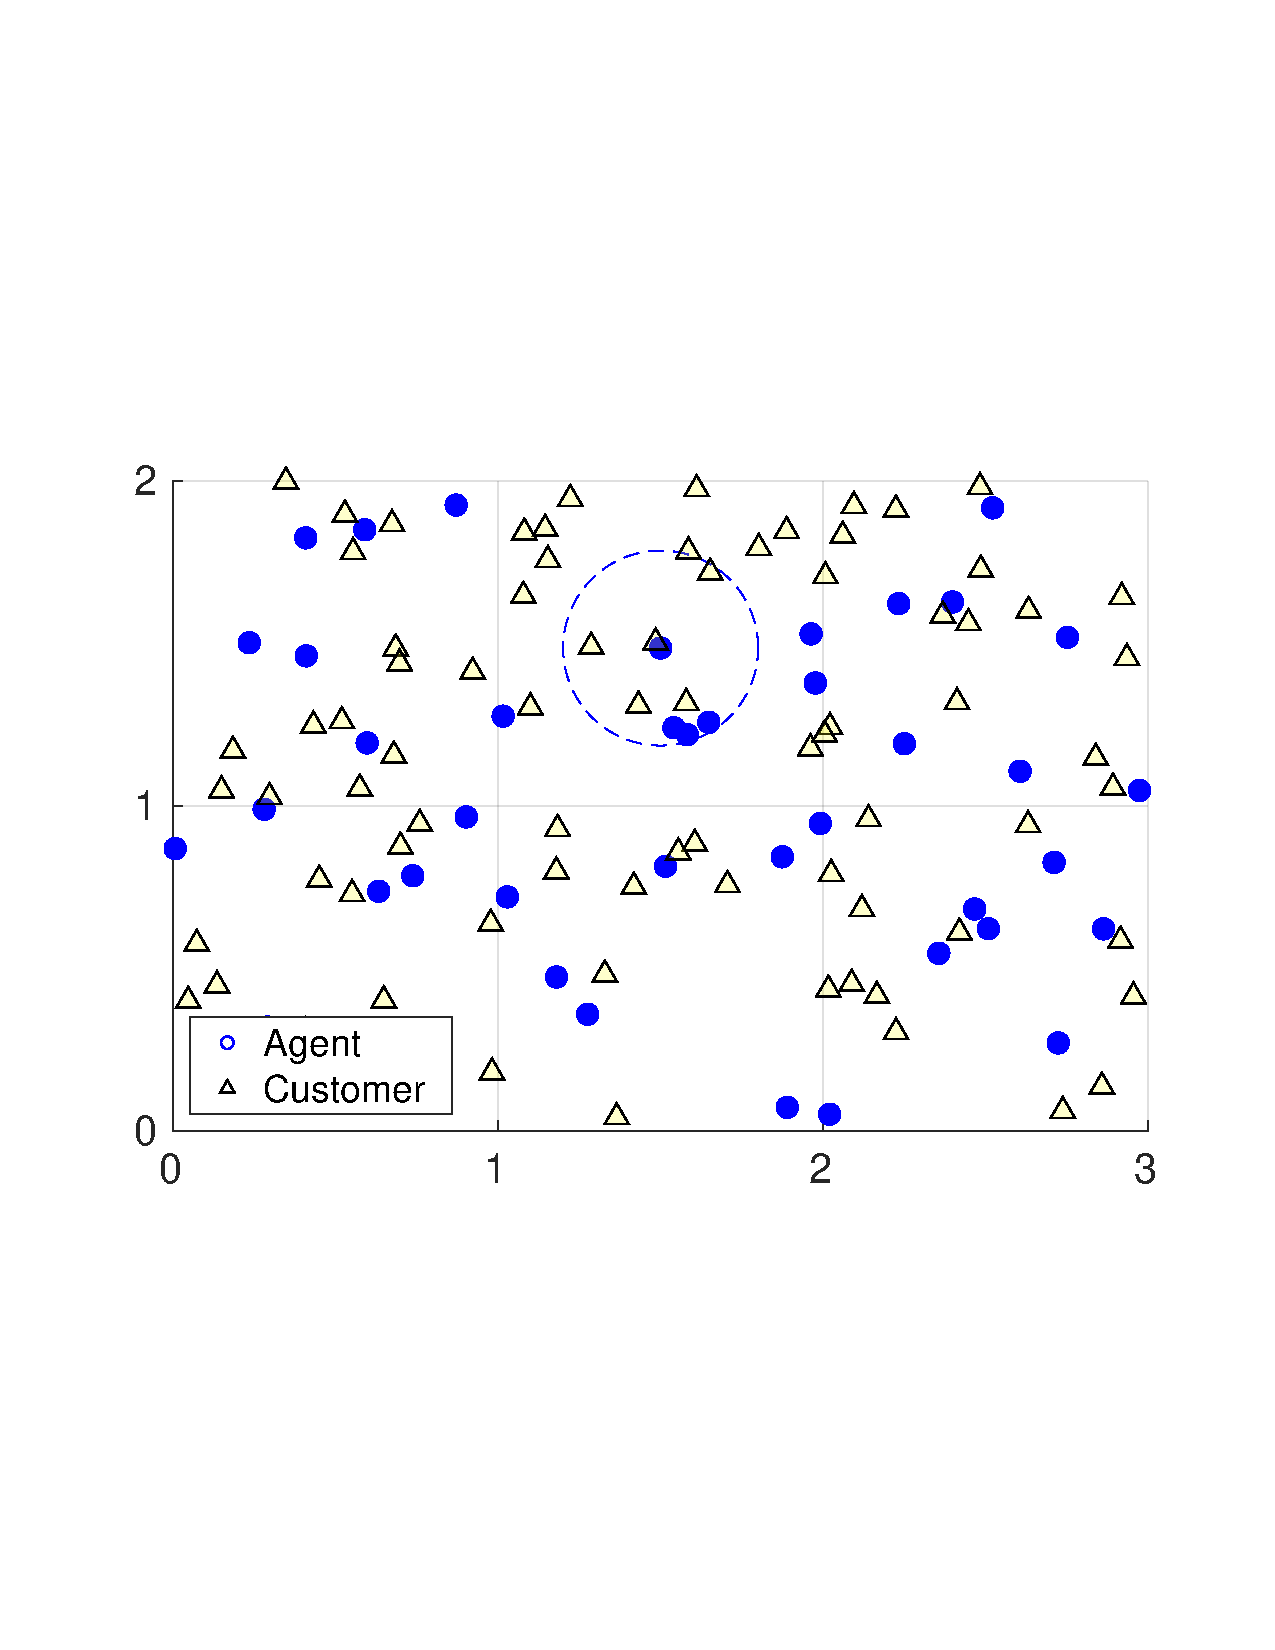
\includegraphics[scale = 0.4, trim={1cm 7.5cm 1cm 7.5cm}, clip]{state_space_3x2.pdf}
    \caption{GridWorld: state space example.}
    \label{fig:state_space_c2}
\end{figure}

\begin{figure}
    \centering
    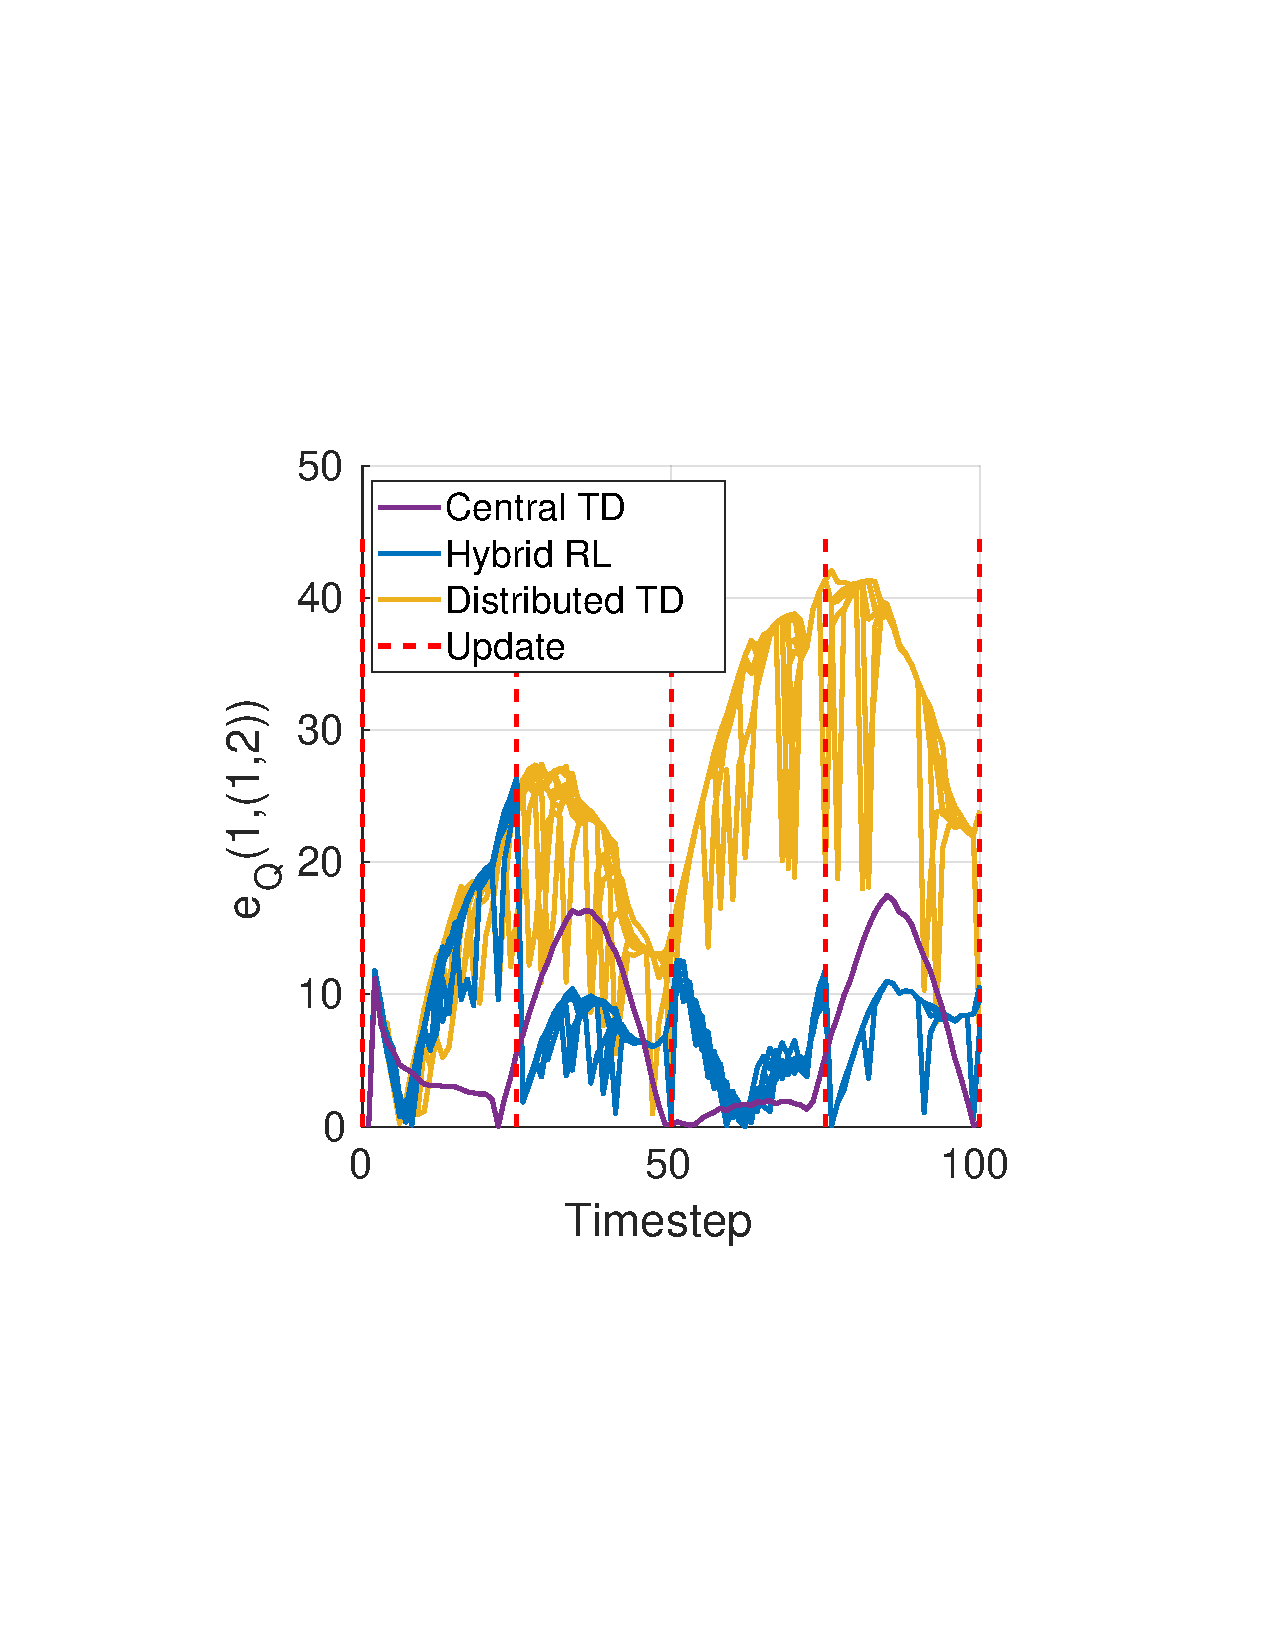
\includegraphics[scale = 0.5, trim={3cm 6.5cm 3cm 7.5cm}, clip]{q_err_track.pdf}
    \caption{GridWorld Q-value error trace with respect to Bellman solution for a single state-action pair.}
    \label{fig:qtrace}
\end{figure}

\begin{figure}
    \centering
    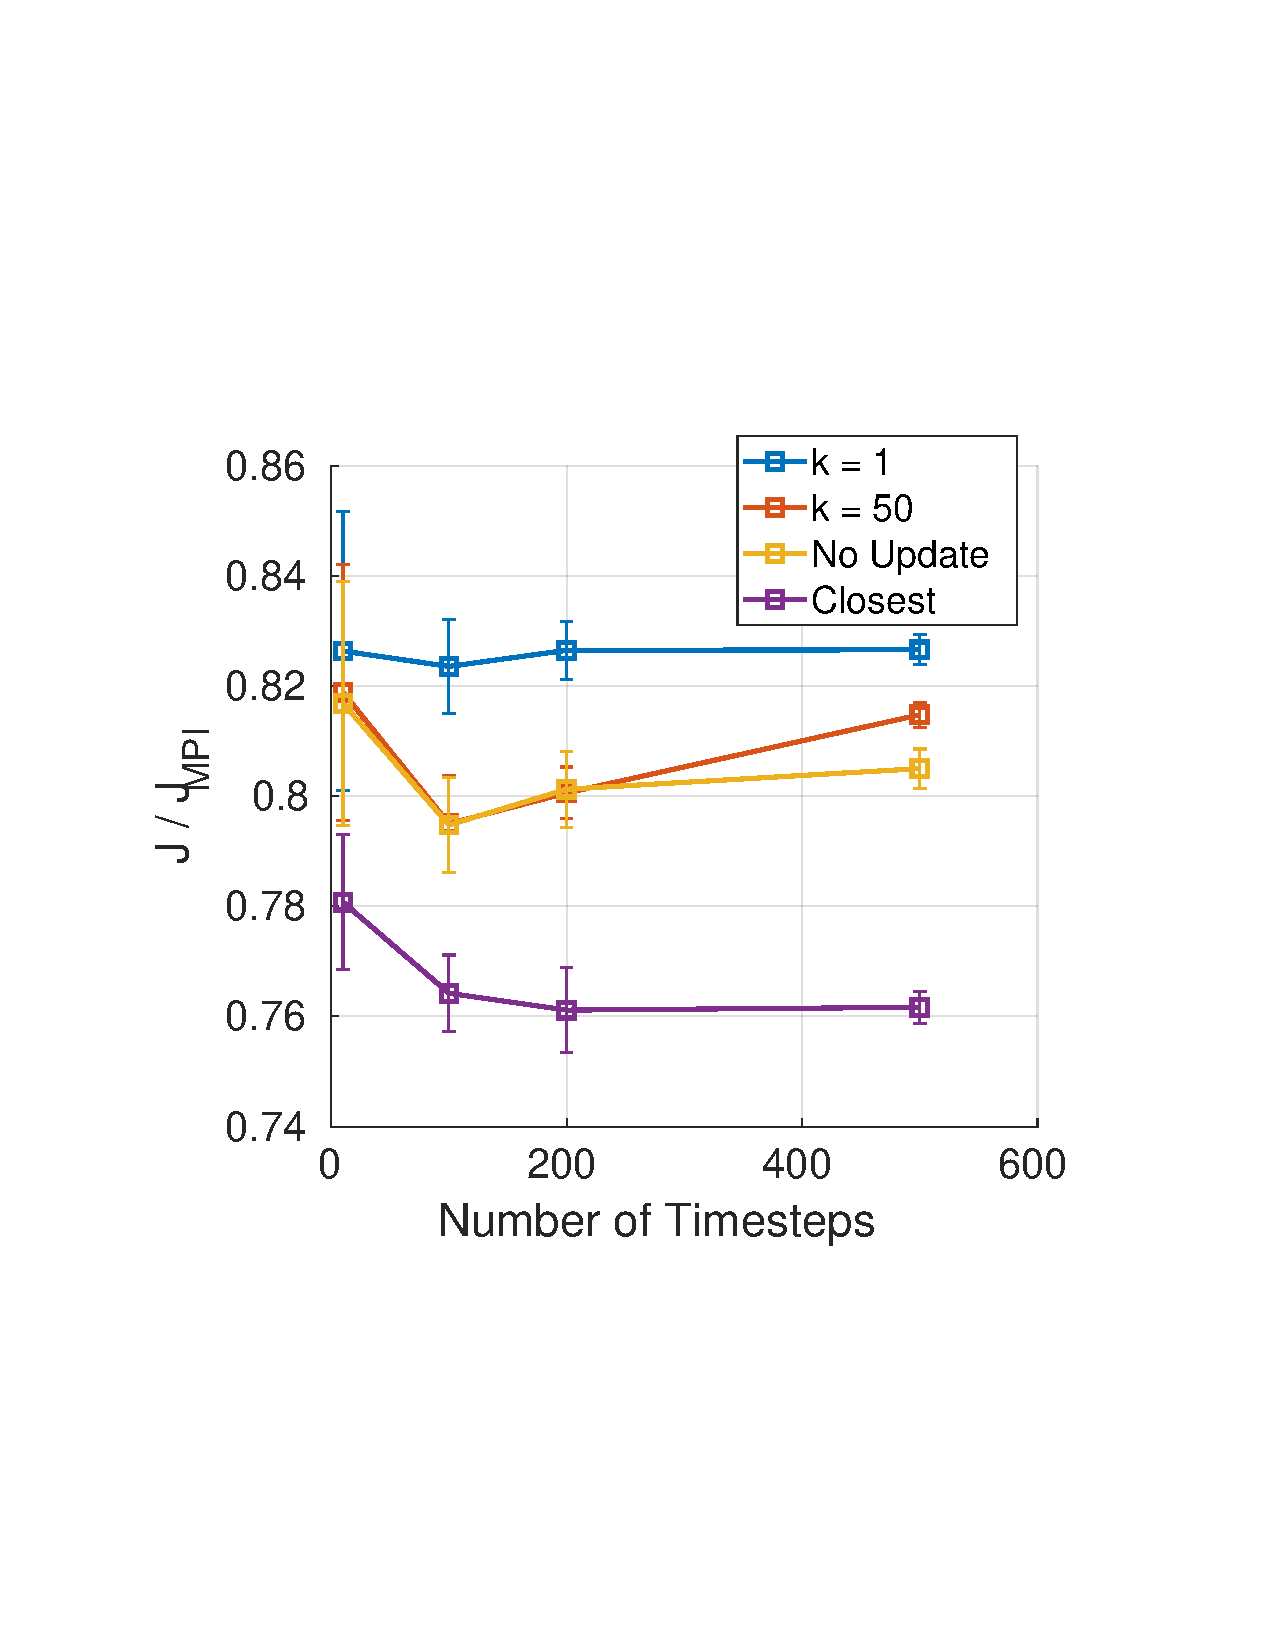
\includegraphics[scale = 0.5, trim={2.5cm 6.5cm 3cm 7cm}, clip]{gridworld_performance_nt_v3.pdf}
    \caption{GridWorld: performance vs. number of time steps for 80 Agents.}
    \label{fig:dist_performance_nt}
\end{figure}

\begin{figure}
    \centering
    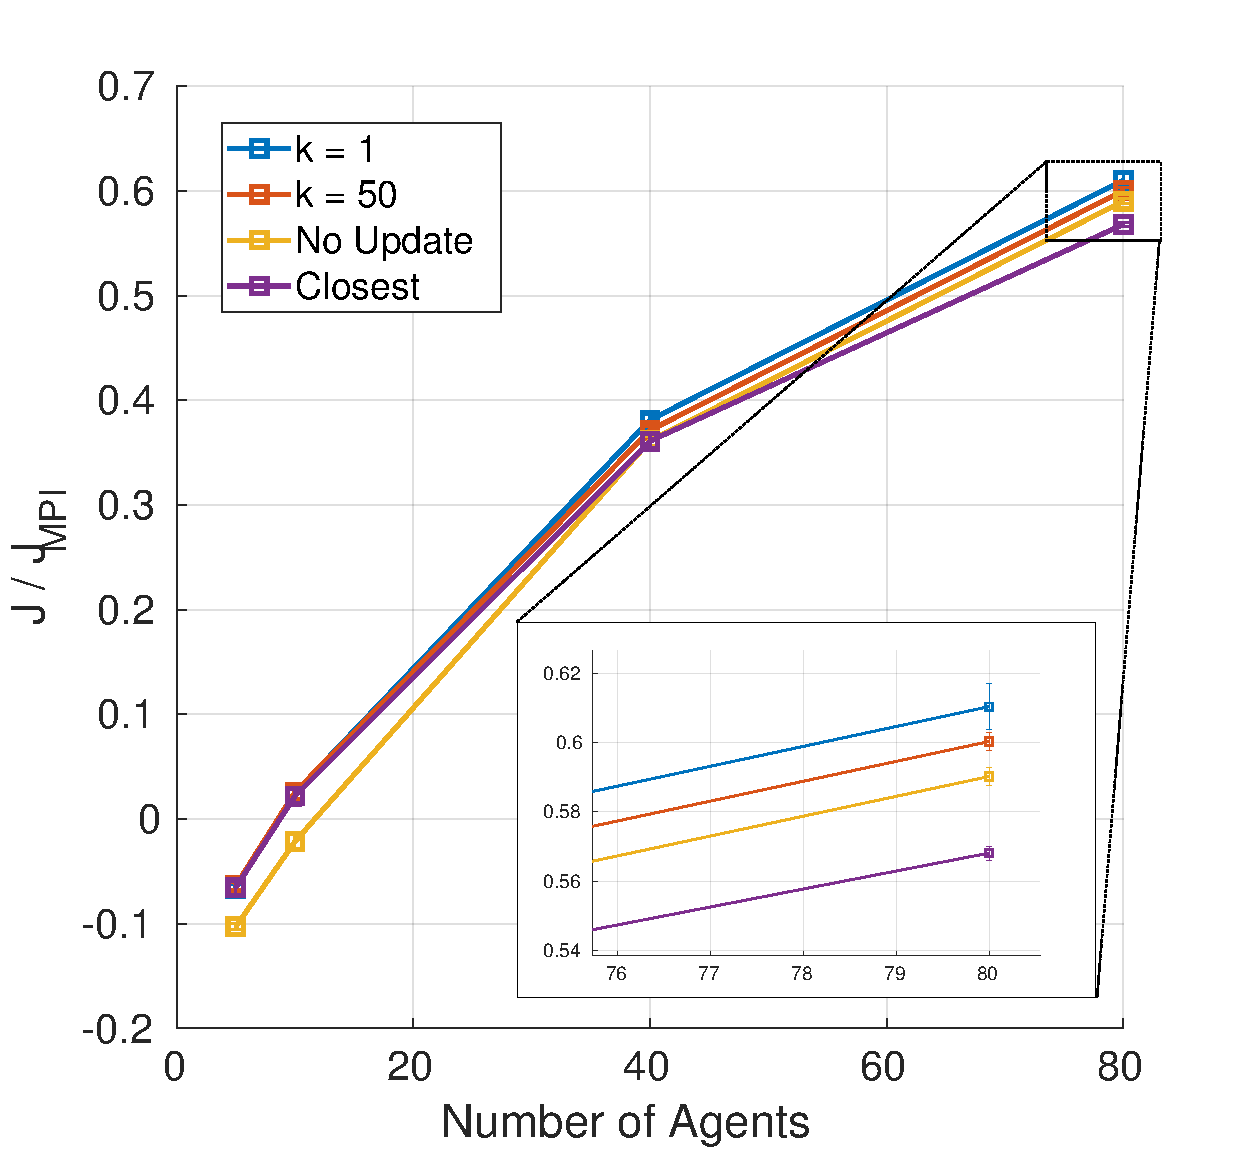
\includegraphics[scale = 0.4, trim={0cm 0cm 0cm 0cm}, clip]{gridworld_dist_performance_ni_v4.pdf} 
    \caption{GridWorld: performance vs. number of agents for 500 time steps.}
    \label{fig:dist_performance_ni}
\end{figure}


\begin{table}[!t]
    \centering
    \caption{Design Parameters}
    \label{table_design_parameters}
    \begin{IEEEeqnarraybox}[\IEEEeqnarraystrutmode\IEEEeqnarraystrutsizeadd{2pt}{1pt}]{v/c/v/c/v/c/v}
        \IEEEeqnarrayrulerow\\
        &\mbox{Variable Name}&&\mbox{GridWorld Value}&&\mbox{Chicago Sim Value}&\\
        \IEEEeqnarraydblrulerow\\
        \IEEEeqnarrayseprow[3pt]\\
        & C_1 && 1 && 0.01 \text{ USD/s} &\IEEEeqnarraystrutsize{0pt}{0pt}\\
        \IEEEeqnarrayseprow[3pt]\\
        \IEEEeqnarrayrulerow\\
        \IEEEeqnarrayseprow[3pt]\\
        & C_2 && 1 && 0.0001 \text{ deg/s} &\IEEEeqnarraystrutsize{0pt}{0pt}\\
        \IEEEeqnarrayseprow[3pt]\\
        \IEEEeqnarrayrulerow\\
        \IEEEeqnarrayseprow[3pt]\\
        & \delta_\text{desired} && \text{N/A} && 10870 &\IEEEeqnarraystrutsize{0pt}{0pt}\\
        \IEEEeqnarrayseprow[3pt]\\
        \IEEEeqnarrayrulerow\\
        \IEEEeqnarrayseprow[3pt]\\
        & \tau && 1 && 1 &\IEEEeqnarraystrutsize{0pt}{0pt}\\
        \IEEEeqnarrayseprow[3pt]\\
        \IEEEeqnarrayrulerow\\
        \IEEEeqnarrayseprow[3pt]\\
        & \lambda && 0.8 && 0.8 &\IEEEeqnarraystrutsize{0pt}{0pt}\\
        \IEEEeqnarrayseprow[3pt]\\
        \IEEEeqnarrayrulerow\\
        \IEEEeqnarrayseprow[3pt]\\
        & \mathcal{q}_t && 1 && 1 &\IEEEeqnarraystrutsize{0pt}{0pt}\\
        \IEEEeqnarrayseprow[3pt]\\
        \IEEEeqnarrayrulerow\\
        \IEEEeqnarrayseprow[3pt]\\
        & \varsigma_t && 1 && 1&\IEEEeqnarraystrutsize{0pt}{0pt}\\
        \IEEEeqnarrayseprow[3pt]\\
        \IEEEeqnarrayrulerow\\
    \IEEEeqnarrayseprow[3pt]\\
        & \gamma && 0.8 && 0.8 &\IEEEeqnarraystrutsize{0pt}{0pt}\\
        \IEEEeqnarrayseprow[3pt]\\
        \IEEEeqnarrayrulerow\\
        \IEEEeqnarrayseprow[3pt]\\
        & |S| && 6 && 20 &\IEEEeqnarraystrutsize{0pt}{0pt}\\
        \IEEEeqnarrayseprow[3pt]\\
        \IEEEeqnarrayrulerow\\        
        \IEEEeqnarrayseprow[3pt]\\
        & R_c && 0.4 && 3500 \mathrm{m} &\IEEEeqnarraystrutsize{0pt}{0pt}\\
        \IEEEeqnarrayseprow[3pt]\\
        \IEEEeqnarrayrulerow
    \end{IEEEeqnarraybox}
\end{table}

\begin{table}[!t]
    \centering
    \caption{Runtime per Agent (sec)}
    \label{table_runtimes}
    \begin{IEEEeqnarraybox}[\IEEEeqnarraystrutmode\IEEEeqnarraystrutsizeadd{2pt}{1pt}]{v/c/v/c/v/c/v/c/v/c/v}
        \IEEEeqnarrayrulerow\\
        & \mbox{} && n_i = 5 && n_i = 10 && n_i = 40 && n_i = 80 \\
        \IEEEeqnarraydblrulerow\\
        \IEEEeqnarrayseprow[3pt]\\
        & k = 1 && 2.9152 && 2.5735 && 2.2096 && 2.0015 &\IEEEeqnarraystrutsize{0pt}{0pt}\\
        \IEEEeqnarrayseprow[3pt]\\
        \IEEEeqnarrayrulerow\\
        \IEEEeqnarrayseprow[3pt]\\
        & k = 50 && 1.1110 && 0.9230 && 0.8868 && 0.8708 &\IEEEeqnarraystrutsize{0pt}{0pt}\\
        \IEEEeqnarrayseprow[3pt]\\
        \IEEEeqnarrayrulerow \\
        \IEEEeqnarrayseprow[3pt]\\
        & \mbox{No Update} && 1.0952 && 0.9449 && 0.8640 && 0.8361 &\IEEEeqnarraystrutsize{0pt}{0pt}\\
        \IEEEeqnarrayseprow[3pt]\\
        \IEEEeqnarrayrulerow
    \end{IEEEeqnarraybox}
\end{table}

\subsection{Chicago City Taxi Simulations}
In this section, we explore the practical applicability of our algorithm by running our simulation using the Chicago city taxi dataset~\cite{chicagoData} for customer requests. The state space of the Chicago map is shown in Fig~\ref{fig:chicago_ss}. As a benchmark for our algorithm, we use the same 'closest' baseline as in the GridWorld simulations. We compute an offline solution using the final hour of April 31, 2017, and our online testing set is over the 24 hours of May 1, 2017 for a total of 17,165 customer requests. We assign a fleet of 100 taxis, and a update condition of $\delta_\mathrm{desired} = 10870$, which corresponds to roughly 10 percent error per Q-value. We choose the design constants, $C_1$ to be 1 cent per second and $C_2$ to be approximately $10$ meters per second, which corresponds to $0.0001$ degrees latitude/longitude per second. The plot of cumulative rewards is shown in Fig.~\ref{fig:chicago_cumulative_rewards}, and it can be seen that our algorithm outperforms the closest and distributed with no update baselines. In total, our distributed algorithm outperformed the `closest' solution by 17.2 percent, which in this case corresponds to 58 USD per taxi per day. It is interesting to note that the slope of the rewards: slow in the early hours of the morning (0 AM--5 AM), then picks up strongly in midday (10 AM--3 PM) and stabilizes to approximately linear for the rest of the day. 

It is important to note the spatial distribution of requests of this dataset, presented in Fig.~\ref{fig:chicago_customer_heatmap}. We can see the cluster of customer requests in the spatial area surrounding near north-side Chicago. The other trend of note is the isolated cluster of customer requests in the far north-east, that we attribute to the Chicago O'Hare airport traffic. When taxi's service there, the bi-modal spatial distribution of requests causes the taxi's graph to be disconnected, instantly triggering a Bellman update request by the result from Theorem~\ref{result:policy_update}.

\begin{figure}
    \centering
    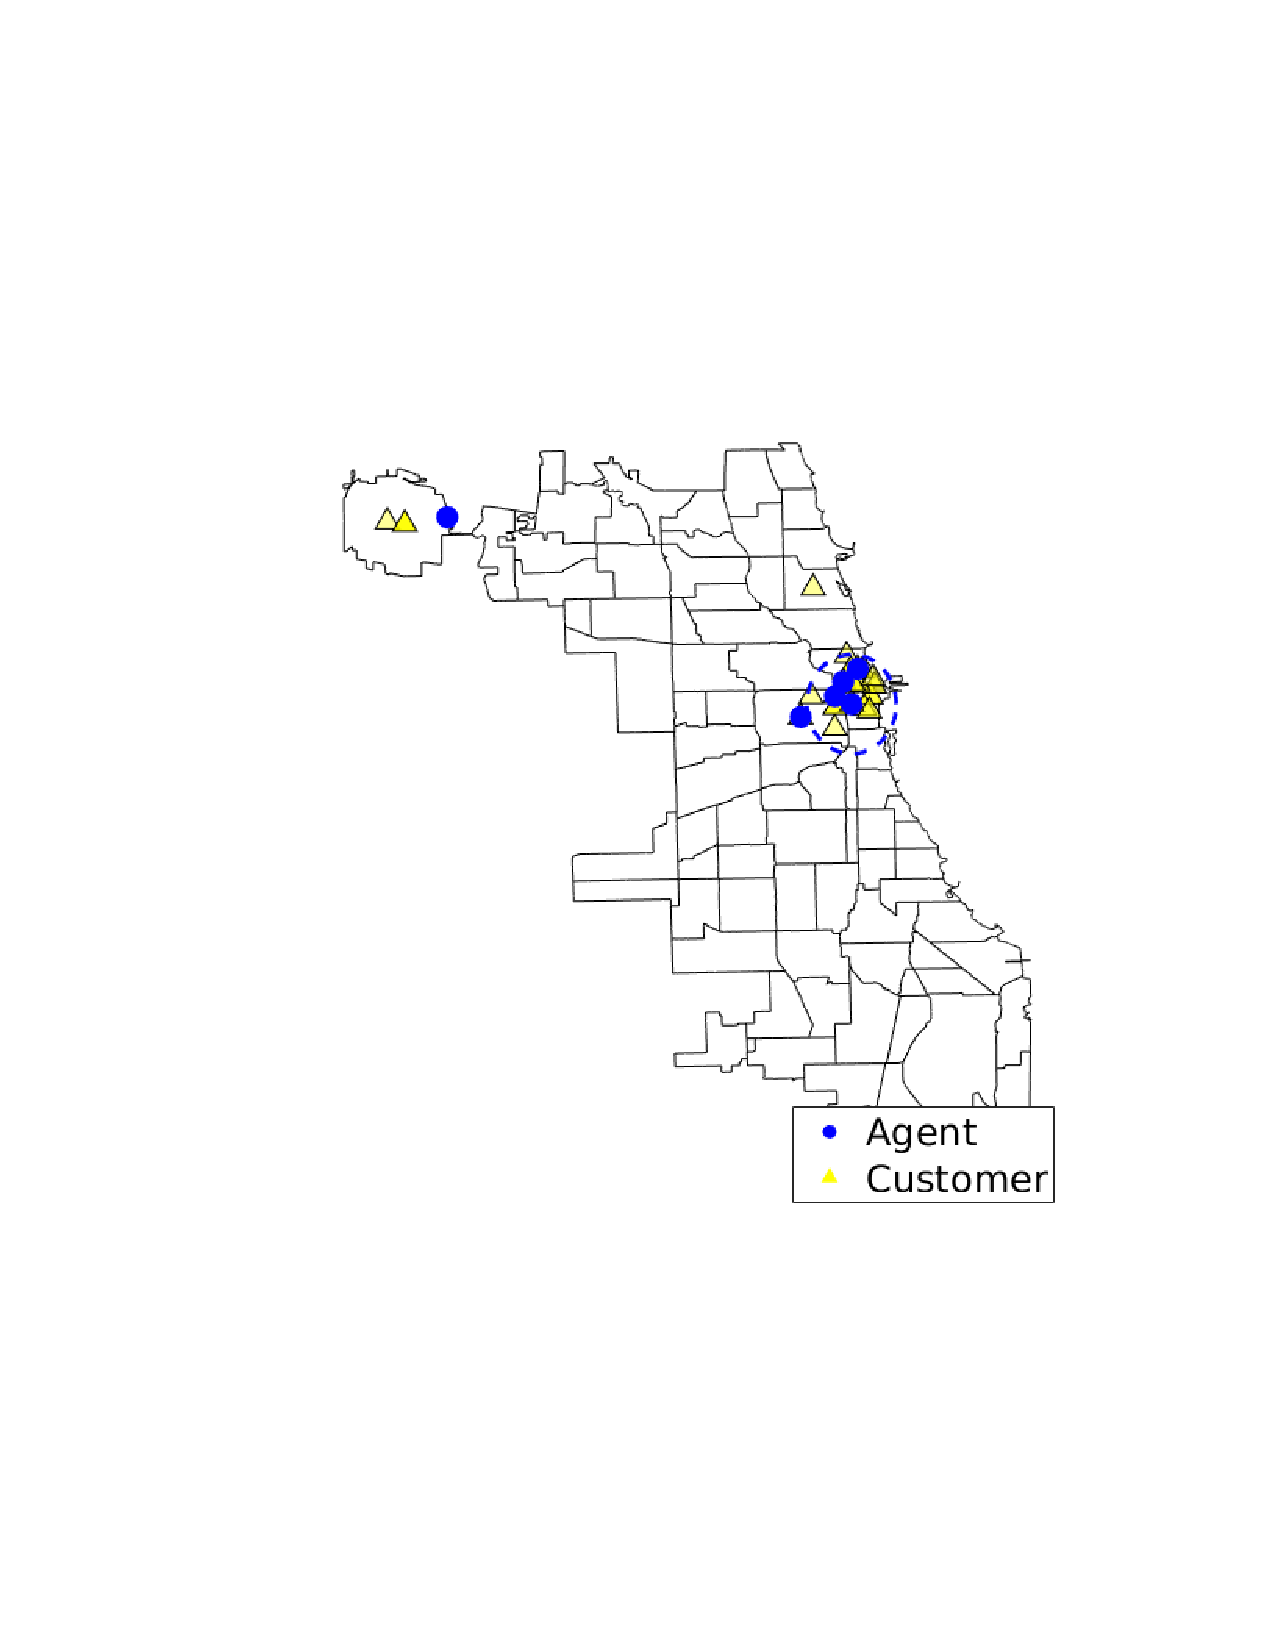
\includegraphics[scale = 0.45, trim={3cm 6cm 0cm 6cm}, clip]{chicago_state_space.pdf}
    \caption{Chicago city state space. Note the bimodal distribution of customer requests at the O-Hare International Airport (northwest), and in the downtown (East).}
    \label{fig:chicago_ss}
\end{figure}

\begin{figure}
    \centering
    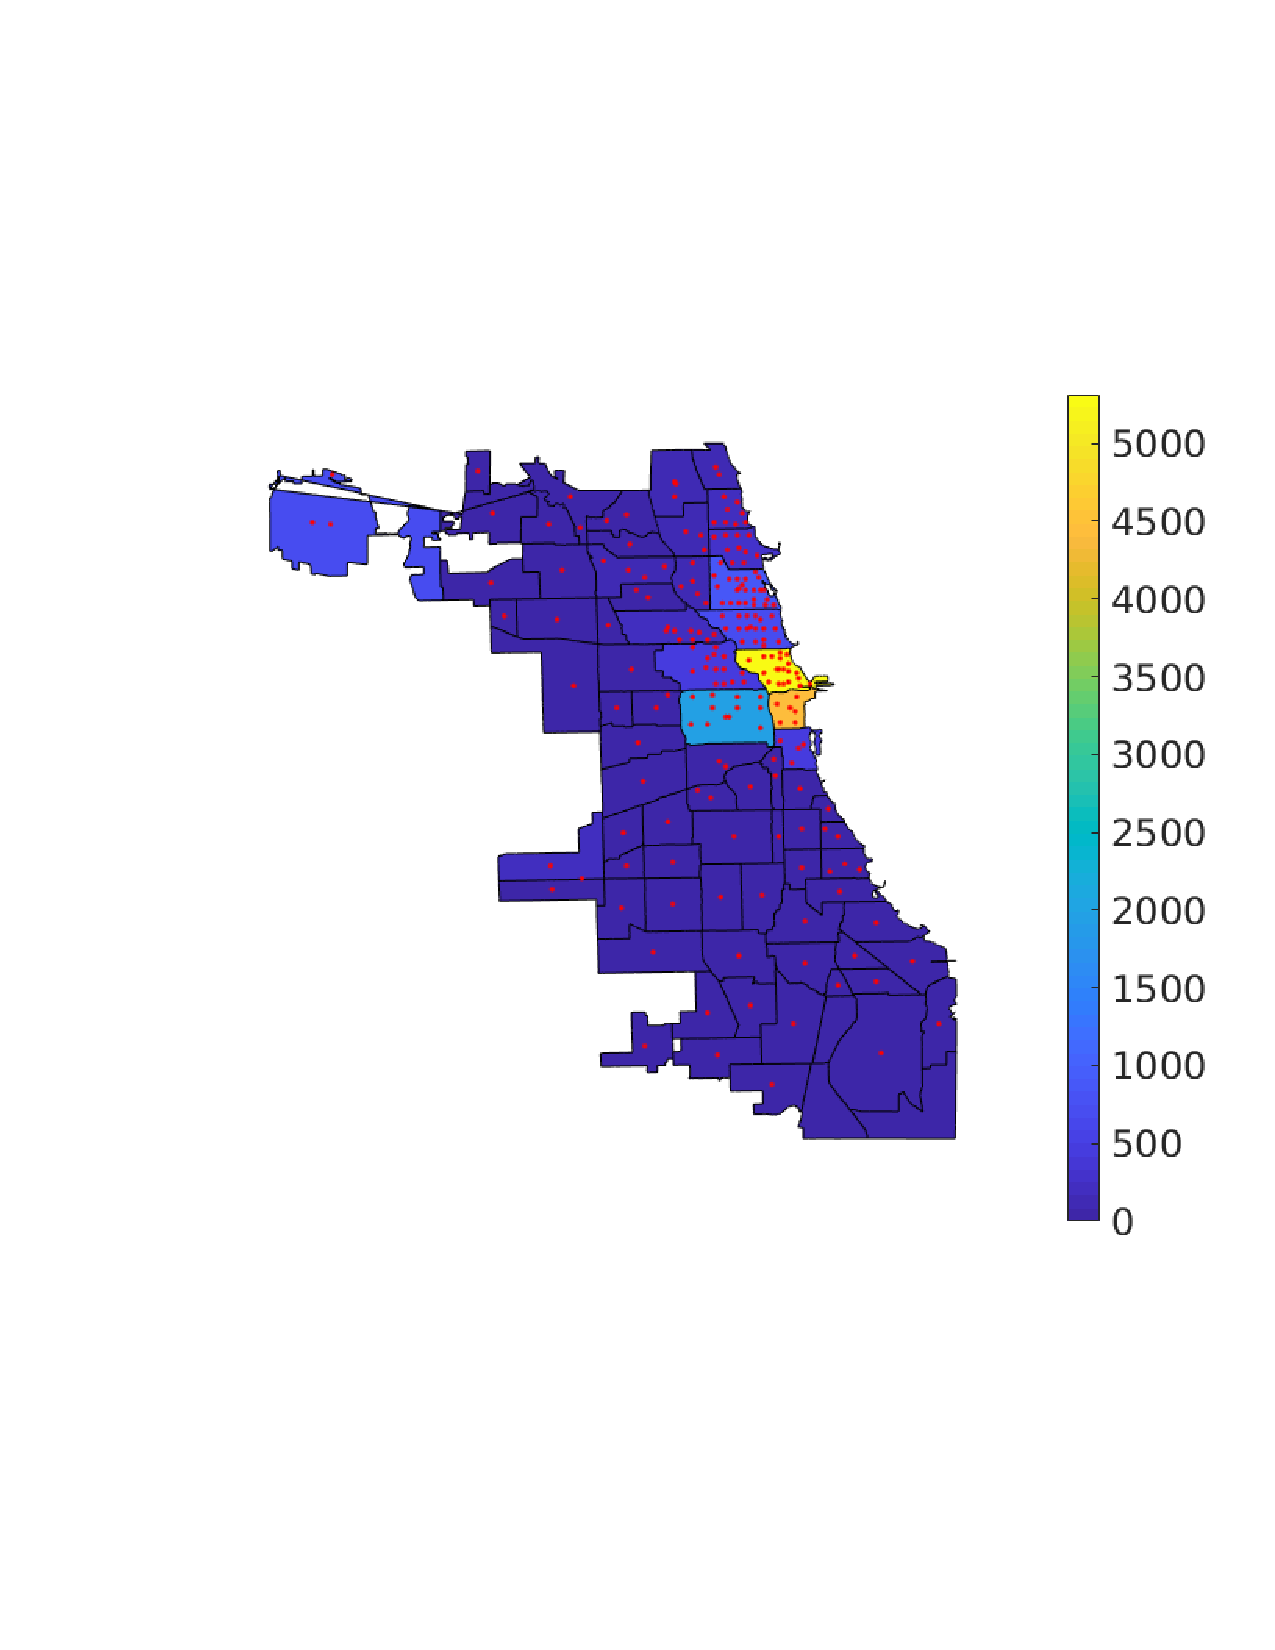
\includegraphics[scale = 0.45, trim={3cm 6cm 0cm 6cm}, clip]{chicago_customer_request_heatmap.pdf}
    \caption{Chicago city customer request heatmap where the red dots represent customer requests.}
    \label{fig:chicago_customer_heatmap}
\end{figure}

\begin{figure}
    \centering
    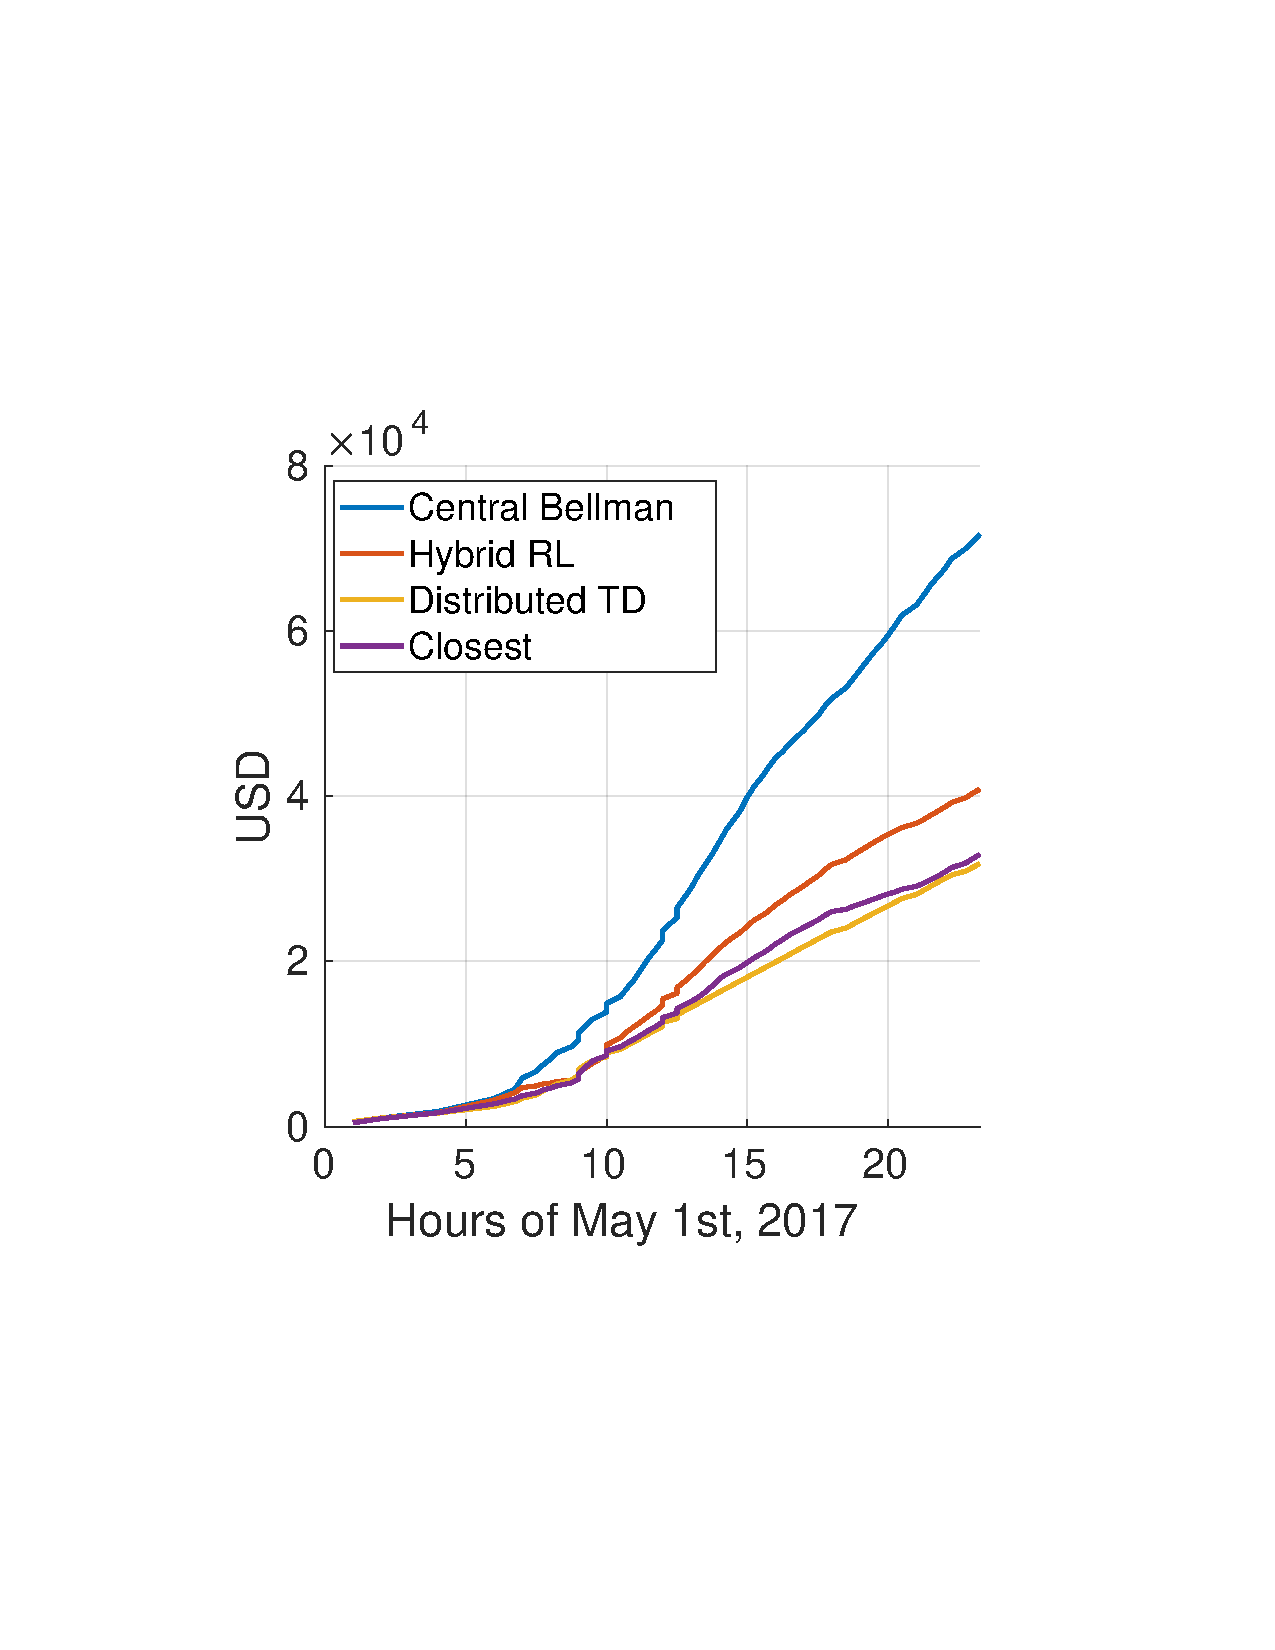
\includegraphics[scale = 0.5, trim={1cm 6cm 1cm 6cm}, clip]{chicago_cumulative_rewards.pdf} 
    \caption{Chicago simulation cumulative rewards for May 1, 2017 for 100 taxis.}
    \label{fig:chicago_cumulative_rewards}
\end{figure}

\section{Conclusion} \label{sec_conclusion}
In this paper, we presented a hybrid distributed reinforcement learning mechanism to solve the urban ride-sharing problem in uncertain and dynamic environments. By formulating an `Eulerian' MDP and distributed reinforcement learning update law, we are able to estimate optimal policy online in a framework that is highly scalable with the number of agents. By exploiting the theoretical intersection of distributed TD Q-learning, Bellman iteration, and distributed estimation analysis from control theory, we are able to provide guarantees on the performance of this method. This allows us to introduce a design constant that characterizes the trade-off of computational expense and estimation accuracy by switching between heavy computations at a central node and light distributed computations at each taxi. We validate our method in a GridWorld environment and using taxi data from the city of Chicago. In the GridWorld environment, we confirmed our theory and expectations by comparing Q-learning and MPI solutions, in centralized and distributed settings. On the real dataset from Chicago city taxis, we found that the proposed algorithm outperforms a closest algorithm by about 17 percent. 
Although our solution is inherently scalable with the number of agents, this formulation is limited with the number of cells in the discretized state-space. Thus, we propose future work in exploring map segmentation, and deep learning methods to reduce the dimensionality. 
Another future direction could be to explore the conventional reward to minimize customer waitng time. We chose to formulate a TNC profit reward function for simplicity and from limitations in the available dataset, but our theoretical framework is compatible with arbitrary reward functions. Finally, we compared our distributed algorithm to a locally greedy algorithm that maximizes reward at each time step. We found that, in some cases, this greedy version would outperform the proposed algorithm, and understanding the performance difference is an ongoing investigation. 

\appendix
\subsection{Contraction Theorems for Discrete Systems}
We present two existing results supporting the proofs of the main theorems.
\begin{theorem}{(Discrete Gronwall Lemma~\cite{stuart_1996})}\label{thm:discrete_gronwall}
    Let a positive sequence $\{Z_n\}$ satisfy:
    \begin{align*}
        Z_{n+1} \leq C Z_n + D \ \ \forall n
    \end{align*}
    for some constants $C, D$, with $C>0$. Then:
    \begin{align*}
        Z_n \leq \frac{ D}{ 1 - C} (1 - C^n) + Z_0 C^n \ \ \forall n
    \end{align*}
    when $C \neq 1$.
\end{theorem}

\subsection{Kalman Information Filter}\label{sec: KIF}
We include the Kalman Information Filter (KIF) form for completeness~\cite{brown_kalman}. 
Consider the following dynamical systems:
\begin{align*}
    x_t &= F_t x_{t-1} + B_t u_t + w_t \\
    z_t &= H_t x_t + v_t 
\end{align*}
where $x_t$ is the hidden state, $z_t$ is the measurement, $F_t$ is the dynamical model, $H$ is the measurement model, $B_t$ is the input matrix, $u_t$ is the input, $w_t$ is the process noise, $w_t \sim N(0, \mathcal{W}_t)$ and $v_t$ is the measurement noise, $v_t \sim N(0, R_t)$. Given these equations, the optimal estimator, $\hat{x}_t$ is given by a prediction and measurement step, that we will write in the notation of the paper. 
The prediction step is given by:
\begin{align*}
    \hat{Q}^i_{t|t-1} &= \hat{Q}^i_{t-1|t-1} \\
    P^i_{t|t-1} &= P^i_{t-1|t-1} + \mathcal{W}_t 
\end{align*}
The measurement step of the information filter is given by defining an information vector, $\hat{y}^i_t$ and information matrix, $Y^i_t$:
\begin{align*}
    Y_{t|t}^i &= (P^i_{t|t})^{-1} \\
    \hat{y}^i_{t|t} &= (P^i_{t|t})^{-1} \hat{Q}^i_{t|t} 
\end{align*}
where measurements $z_t^i$ taken at time step $t$ can be transformed as:
\begin{align*}
    Y^i_{t|t} &= Y^i_{t|t-1} + (H^i_t)^\intercal R_t^{-1} H^i_t \\
    \hat{y}^i_{t|t} &= \hat{y}^i_{t|t-1} + (H^i_t)^\intercal R_t^{-1} z_t^i
\end{align*}
Finally, the Kalman gain, $\alpha^i_t$ is calculated as follows:
\begin{align*}
    S^i_t &= H^i_t P^i_{t|t-1} (H^i_t)^\intercal + R_t \\
    \alpha^i_t &= P^i_{t|t-1} (H^i_t)^\intercal (S^i_t)^{-1}
\end{align*}

% use section* for acknowledgment
\section*{Acknowledgment}
The authors thank the feedback from colleagues in the Data-driven Intelligent Transportation workshop (DIT 2018, held in conjunction with IEEE ICDM). The work is funded in part by the Raytheon Company. 
The authors would also like to thank Wolfgang Hoenig and Anthony Fragoso for their helpful feedback and comments. 

\bibliographystyle{IEEEtran}
\bibliography{IEEEabrv,IEEE_bib2}


\begin{IEEEbiographynophoto}{Benjamin Riviere}
is a PhD student at California Institute of Technology (Caltech). He received the B.S. in Mechanical Engineering from Stanford University in 2017 and the M.S. in Aeronautics from Caltech in 2018. His research interests include combining machine learning and network control theory with applications in transportation and space systems. 
\end{IEEEbiographynophoto}

% % if you will not have a photo at all:
\begin{IEEEbiographynophoto}{Salar Rahili} received the B.S. and the M.Sc. degrees in electrical engineering from the Isfahan University of Technology, Isfahan, Iran, in 2009 and 2012, respectively. He received his Ph.D. degree in electrical engineering at the University of California, Riverside, CA, USA, in 2016 and joined the Aerospace Department of the California Institute of Technology, USA, as a postdoctoral researcher afterwards.  His research focuses on distributed control of multi-agent systems, reinforcement learning, distributed optimization, and guidance and control of autonomous systems. 
\end{IEEEbiographynophoto}

\begin{IEEEbiographynophoto}{Soon-Jo Chung} received the B.S. degree (summa cum laude) from Korea Advanced Institute of Science and Technology, Daejeon, South Korea, in 1998; the S.M. degree in aeronautics and astronautics; and the Sc.D. degree in estimation and control from Massachusetts Institute of Technology, Cambridge, MA, USA, in 2002 and 2007, respectively. He is the Bren Professor of Aerospace and Jet Propulsion Laboratory Research Scientist in the California Institute of Technology. Dr. Chung was on the faculty of the University of Illinois at Urbana-Champaign (UIUC) during 2009-2016. His research focuses on spacecraft and aerial swarms and autonomous aerospace systems, and in particular, on the theory and application of complex nonlinear dynamics, control, estimation, guidance, and navigation of autonomous space and air vehicles. Dr. Chung is received the UIUC Engineering Deans Award for Excellence in Research, the Beckman Faculty Fellowship of the UIUC Center for Advanced Study, the U.S. Air Force Office of Scientific Research Young Investigator Award, the National Science Foundation Faculty Early
Career Development Award, and three Best Conference Paper Awards from the IEEE, and the American Institute of Aeronautics and Astronautics. He is an Associate Editor of IEEE Transactions on Robotics, IEEE Transactions on Automatic Control, and Journal of Guidance, Control, and Dynamics.
\end{IEEEbiographynophoto}

\end{document}



